\documentclass[letterpaper,twocolumn,10pt]{article}
\usepackage{usenix-2020-09}
\usepackage{ragged2e}
\hbadness=10000
\hfuzz=8pt
\usepackage{placeins}
\usepackage{amsmath,amssymb,mathtools,amsthm}
\usepackage[hypcap=false]{caption}
\usepackage{booktabs,multirow,graphicx,framed}
\usepackage[advantage,adversary,notions,probability,events,complexity]{cryptocode}
\usepackage{algorithm}
\usepackage{algorithmic}

\emergencystretch=1.5em

\newtheorem{theorem}{Theorem}
\newtheorem{lemma}[theorem]{Lemma}
\newtheorem{corollary}[theorem]{Corollary}
\theoremstyle{definition}
\newtheorem{definition}[theorem]{Definition}

\newcommand{\B}{\mathbb{B}}
\newcommand{\Z}{\mathbb{Z}}\newcommand{\N}{\mathbb{N}}
\newcommand{\U}{\mathcal{U}}\newcommand{\cF}{\mathcal{F}}
\newcommand{\cL}{\mathcal{L}}\newcommand{\cS}{\mathcal{S}}
\newcommand{\cA}{\mathcal{A}}\newcommand{\cB}{\mathcal{B}}\newcommand{\cZ}{\mathcal{Z}}
\newcommand{\prm}{\mathsf{prm}}\newcommand{\Enc}{\mathsf{Enc}}
\newcommand{\Dec}{\mathsf{Dec}}\newcommand{\Encode}{\mathsf{Encode}}
\newcommand{\DeleteSet}{\mathsf{DeleteSet}}\newcommand{\Peel}{\mathsf{Peel}}
\newcommand{\List}{\mathsf{List}}\newcommand{\uPeel}{\mathsf{uPeel}}
\newcommand{\PRF}{\mathsf{PRF}}\newcommand{\SE}{\mathsf{SE}}
\newcommand{\Adv}{\mathsf{Adv}}\newcommand{\negl}{\mathsf{negl}}\newcommand{\poly}{\mathsf{poly}}
\newcommand{\sample}{\leftarrow_{\$}}\newcommand{\concat}{\|}

\begin{document}
\title{Forward-Private Updatable Private Set Union from Incremental IBLT Encoding}
\author{Anonymous Submission}
\maketitle

\begin{abstract}
Private Set Union (PSU) enables two parties to compute the union of their
private sets. While recent IBLT-based protocols achieve PSU performance
competitive with Private Set Intersection, they are \emph{static}: computing the
union on updated sets requires re-running the full protocol from scratch.

We present \textbf{FUPSU}, the first forward-private updatable PSU protocol.
FUPSU exploits the linearity of IBLT encoding to support incremental
(delta-based) set updates, achieving per-epoch communication and computation
$O(|\Delta|)$. We identify and resolve a fundamental barrier to IBLT-based
incremental updates: \emph{deletion cascade}, where removing even a few elements
triggers global propagation through the IBLT structure, erasing the benefit of
incremental processing. Our key insight---\textbf{OT-masked deletion}---offloads
deletion membership checks to Oblivious Transfer, preventing shared-element
deletions from entering the IBLT cascade path entirely. This restores true
$O(|\Delta|)$ scaling, yielding $29$--$23{,}756\times$ per-epoch cell scan
reduction over static full re-encoding, across update sizes $|\Delta|=64$--$4096$.
Forward privacy is obtained via a PRF-based key evolution chain with immediate
erasure, adding negligible overhead. We also prove a \emph{leakage lower bound}:
any updatable PSU protocol with sublinear communication must leak individual
add and delete counts---our protocol matches this bound and is therefore
leakage-optimal.

We further show that a single execution of the UnionPeel sub-protocol
simultaneously recovers the union, the intersection, and their
cardinalities---yielding a \emph{unified} updatable private set operation
framework (updPSO) with zero additional communication or computation.
We implement FUPSU end-to-end in C++ and benchmark across set sizes $2^{14}$
to $2^{20}$ with $100\%$ recovery across all configurations. All code is
open source.
\end{abstract}

\section{Introduction}
% ============================================================

Private Set Union (PSU)~\cite{KRT19,JLZ20,ZCL+23,Tu+25} allows two parties to
compute the union $X \cup Y$ of their private sets while revealing nothing
beyond the union itself. With applications in privacy-preserving identity
management, collaborative cyber-risk assessment, private database joins, and
federated learning~\cite{DCW13,IKN+20,KRS+19}, PSU is a fundamental secure
computation primitive alongside Private Set Intersection (PSI).

Historically, PSU has been significantly slower than PSI---often by $30\times$
or more~\cite{PT26,KRT19}. The recent breakthrough of Piske and
Trieu~\cite{PT26} (Eurocrypt 2026) closed this gap by introducing the first
IBLT-based PSU protocol. Their key insight, \emph{union peelability}, enables
peeling the union of two IBLTs without materializing the combined table, using
oblivious transfer (OT) and an oblivious PRF (OPRF). The resulting protocol
computes PSU on $2^{20}$ elements in under 3 seconds, matching state-of-the-art
PSI performance.

\textbf{The static limitation.} Piske and Trieu's protocol, like all prior PSU
constructions, is \emph{static}: both parties must encode their entire sets into
fresh IBLTs for each computation. In many real-world applications, however,
sets evolve incrementally---new elements are added, old ones expire---in applications
including threat intelligence sharing, federated learning with evolving client
datasets, and private database join maintenance under incremental updates.
Re-running the full protocol on each update wastes resources proportional
to the total set size, even when only a handful of elements change.

\textbf{The forward privacy requirement.} The multi-epoch nature of updatable
protocols introduces a new security concern: \emph{forward privacy}. If a party
is compromised at epoch $\tau$, the adversary should not be able to recover the
party's historical set elements from epochs $t < \tau$, even having observed all
protocol messages. This is the privacy analogue of forward secrecy in
Signal~\cite{Signal}, and is critical when sets contain sensitive data with
limited lifetimes. Privacy regulations (GDPR, CCPA) mandate data retention
limits; if historical elements remain decryptable after key compromise, the
system violates the principle that deleted data should be irrecoverable.

\textbf{Existing updatable work.} Several updatable PSI protocols
exist~\cite{BMX22,BMS+24,LMR+26,ABF+25,LTS+26}, with FUPSI~\cite{WZC+24}
achieving forward privacy via keyword PIR. \textbf{No prior work} addresses updatable PSU,
let alone forward-private updatable PSU.

\textbf{Our contributions.} We initiate the study of updatable PSU with forward
privacy:

\begin{enumerate}
\item \textbf{The FUPSU protocol} (Section~\ref{sec:protocol}). The first
forward-private updatable PSU protocol. Built on three mechanisms: (i)~delta IBLT
encoding with $O(|\Delta|)$ per-epoch cell operations;
size $n$; (ii)~\textbf{OT-masked deletion}, which offloads deletion membership
checks to Oblivious Transfer, preventing shared-element deletions from entering
the IBLT cascade path; (iii)~split-path incremental peeling with cascade bounded
by $2k|\Delta|$; (iv)~PRF-based key evolution for forward privacy. UnionPeel
simultaneously recovers the intersection and cardinalities, yielding a unified
updPSO framework.

\item \textbf{Leakage lower bound} (Section~\ref{sec:protocol}, Theorem~\ref{thm:lower}). We prove that
\emph{any} $1$-updatable PSU protocol must reveal the individual add and delete
counts for each party---an inherent efficiency-leakage trade-off. Any protocol
hiding these counts requires $\Omega(N\sigma)$ communication, defeating
updatability. FUPSU's OT queries and delta IBLT sizes reveal these four counts,
matching the lower bound and making it \textbf{leakage-optimal}.

\item \textbf{Implementation and evaluation} (Section~\ref{sec:eval}).
We implement FUPSU end-to-end in C++ (IBLT with $k{=}5$, OT-masked deletion,
MiniPeel for additions). Benchmarks on Intel Xeon E5-2630 v4 across set sizes
$2^{14}$--$2^{20}$ and update sizes $|\Delta|=64$--$4096$ achieve
$29$--$23{,}756\times$ per-epoch cell scan reduction over static full
re-encoding, with $100\%$ recovery across all configurations. We identify
the deletion cascade barrier and quantify how OT-masking eliminates it.
\end{enumerate}

\smallskip\noindent
On the security front, we prove FUPSU UC-realizes~\cite{Can01}
$\cF_{\mathsf{updPSU}}$ in the $(\cF_{\mathsf{OPRF}},
\cF_{\mathsf{OT}})$-hybrid model against semi-honest adaptive adversaries,
with a modular proof that separates per-epoch PSU security from cross-epoch
key management, enabling independent upgrades. We introduce FP-IND, a
standalone game-based definition that cleanly captures the forward privacy
guarantee of the PRF chain. Because PSU outputs the union, FUPSU is
structurally unaffected by adaptive input-selection attacks
on UPSI~\cite{LMR+26}, requiring no protocol modification.

\smallskip
\noindent\textbf{Comparison with prior work.}
Table~\ref{tab:intro-compare} situates FUPSU among prior PSU and
updatable protocols.

\begin{table*}[t]
\centering
\footnotesize
\begin{tabular}{|l|l|c|c|c|c|c|}
\hline
\textbf{Protocol} & \textbf{Type} & \textbf{Updatable} & \textbf{Fwd.\ Priv.} & \textbf{UC} & \textbf{Adaptive} & \textbf{Complexity} \\
\hline\noalign{\vspace{-1pt}}\hline
KRT19~\cite{KRT19}   & PSU & No  & No  & Yes & No  & $O(n)$ \\
ZCL+23~\cite{ZCL+23} & PSU & No  & No  & Yes & No  & $O(n)$ \\
Jia+24~\cite{Jia+24} & PSU & No  & No  & Enhanced & No  & $O(n \log n)$ \\
Tu+25~\cite{Tu+25}   & PSU & No  & No  & Enhanced & No  & $O(n)$ \\
PT26~\cite{PT26}     & PSU & No  & No  & Yes & No  & $O(n)$ \\
FUPSI~\cite{WZC+24}  & PSI & Yes & Yes & No  & No  & $O(\log n)$ \\
LMR+26~\cite{LMR+26} & PSI & Yes & No  & Yes & Yes & $O(|\Delta|)$ \\
\hline\noalign{\vspace{-1pt}}\hline
\textbf{Ours} & PSU & Yes & Yes & Yes & Yes & $O(|\Delta|)$ \\
\hline
\end{tabular}

\smallskip
\caption{Comparison with prior PSU and updatable protocols.
Enhanced = UC-secure under the enhanced PSU functionality (no within-execution leakage).}
\label{tab:intro-compare}
\end{table*}

% ============================================================

\subsection{Technical Overview}

We now give an informal walkthrough of our key technical ideas. The formal protocol specification appears in Section~\ref{sec:protocol}, with full proofs in Sections~\ref{sec:security} and the Appendix.

\subsubsection{The Deletion Cascade Barrier}\label{sec:cascade-barrier}

A natural incremental approach applies delta IBLT encoding: deletions are
subtracted from IBLT cells, and UnionPeel starts from the $k|\Delta^-|$
modified cells. This directly realizes the Cascade Bound Lemma
(Lemma~\ref{lem:cascade}), which proves $\leq 2k|\Delta^-|$ cells are
examined. However, \emph{in practice}, the cascade does not stop there.

The issue is structural. After subtracting deleted elements, new singletons
emerge in the IBLT. Peeling these singletons exposes further singletons---a
chain reaction that propagates through \emph{all remaining shared elements}
in the IBLT, not just those related to deletions. Empirically, a single
deletion sweep peels $\approx 70$--$80\%$ of all shared elements, examining
$\Theta(|S|)$ cells instead of $O(|\Delta|)$. This reduces the incremental
benefit to only $6$--$10\times$ over static re-encoding, far below the
theoretical $n/|\Delta|$ potential.

\subsubsection{OT-Masked Deletion}

Our key insight is that \emph{most deletions do not require IBLT
modification at all}. When a party deletes an element $x$, the protocol
only needs to know whether $x$ is (i)~unique to the deleting party,
(ii)~shared but retained by the other party, or (iii)~deleted by both.
Using a 2-bit OT-based membership check---already supported by the
$\cF_{\mathsf{OPRF}}$ and $\cF_{\mathsf{OT}}$ functionalities used by
UnionPeel---the parties classify each deletion into one of three cases:

\begin{itemize}
\item \textbf{Case~1 (unique):} The other party does not hold $x$. The element
  is removed from the union via local update only---no IBLT modification.
\item \textbf{Case~2 (one-sided shared):} The other party holds $x$ and does
  not delete it. $x$ remains in the union. The deleting party subtracts $x$
  from its IBLT ($k$ cell updates, no cascade).
\item \textbf{Case~3 (two-sided shared):} Both parties independently delete
  $x$. This is the only case requiring IBLT subtraction ($\ominus$~on both
  parties' IBLTs).
\end{itemize}

In practice, Case~3 is rare ,
because the probability of both parties independently selecting the same
shared element for deletion is low. The remaining deletions are
handled purely locally (Case~1) or via OT without IBLT touch (Case~2). This
\emph{eliminates deletion cascade entirely}---per-epoch cell scanning is
dominated by the Mini UnionPeel for additions, at $O(|\Delta^+|)$ cells.
The resulting per-epoch cost is true $O(|\Delta|)$, restoring the full
$n/|\Delta|$ reduction factor.
\section{Preliminaries}
\label{sec:overview}
% ============================================================

\subsection{Invertible Bloom Lookup Tables}

Invertible Bloom Lookup Tables (IBLTs) were introduced by Goodrich and
Mitzenmacher~\cite{GM11}. An IBLT is a variant of Bloom filter that supports,
in addition to inserting and deleting elements, the ability to \emph{list} all
stored elements. Unlike a standard Bloom filter---which only answers membership
queries with a configurable false-positive rate and requires $\approx 60\times$
expansion for negligible error---an IBLT stores key-value pairs in its cells
and achieves listing with expansion factor $1.5$--$4.5\times$ (for $k = 4$ hash
functions). This makes IBLTs uniquely suited for set reconciliation and private
set union, where the goal is to recover the entire set rather than answer
individual membership queries.

An IBLT is parameterized by $\prm = (M, k, \ell, H)$: a modulus $M \in
\N_{\geq 2}$ (typically $2^{64}$), $k$ hash functions $H = \{h_i : \U \to
[\ell]\}_{i \in [k]}$ each mapping to a distinct subtable of size $\ell$, and
two $k \times \ell$ matrices $\mathsf{sum}$ (values in $\Z_M$) and
$\mathsf{cnt}$ (non-negative integers). We write $m = k\ell$ for the total
number of cells.

The three core operations are given in Algorithms~\ref{alg:encode}--\ref{alg:list}.

\begin{algorithm}[ht]
\caption{$\Encode_{\prm}(X)$ --- IBLT encoding.}
\label{alg:encode}
\begin{algorithmic}
\STATE \textbf{Input:} $\prm = (M, k, \ell, H)$, set $X \subseteq \U$, empty IBLT $(\mathsf{sum}, \mathsf{cnt})$.
\STATE \textbf{Output:} $\mathsf{IBLT} = (\mathsf{sum}, \mathsf{cnt}, \prm)$ containing all $x \in X$.
\STATE Initialize $\mathsf{sum}[i][j] \leftarrow 0$, $\mathsf{cnt}[i][j] \leftarrow 0$ for all $i \in [k], j \in [\ell]$.
\FOR{each $x \in X$}
  \FOR{$i \in [k]$}
    \STATE $j \leftarrow h_i(x)$
    \STATE $\mathsf{sum}[i][j] \leftarrow \mathsf{sum}[i][j] + x \pmod M$
    \STATE $\mathsf{cnt}[i][j] \leftarrow \mathsf{cnt}[i][j] + 1$
  \ENDFOR
\ENDFOR
\end{algorithmic}
\end{algorithm}

\begin{algorithm}[ht]
\caption{$\DeleteSet_{\prm}(\mathsf{IBLT}, X)$ --- batch deletion.}
\label{alg:deleteset}
\begin{algorithmic}
\STATE \textbf{Input:} $\mathsf{IBLT} = (\mathsf{sum}, \mathsf{cnt}, \prm)$ and set $X \subseteq \U$.
\STATE \textbf{Output:} Updated $\mathsf{IBLT} = (\mathsf{sum}, \mathsf{cnt}, \prm)$ with all $x \in X$ removed.
\FOR{each $x \in X$}
  \FOR{$i \in [k]$}
    \STATE $j \leftarrow h_i(x)$
    \STATE $\mathsf{sum}[i][j] \leftarrow \mathsf{sum}[i][j] - x \pmod M$
    \STATE $\mathsf{cnt}[i][j] \leftarrow \mathsf{cnt}[i][j] - 1$
  \ENDFOR
\ENDFOR
\end{algorithmic}
\end{algorithm}

IBLT encoding is \emph{linear}: $\Encode(A \cup B) = \Encode(A) \oplus
\Encode(B)$ and $\Encode(A \setminus B) = \Encode(A) \ominus \Encode(B)$,
where $\oplus$/$\ominus$ denote cell-wise modular addition/subtraction.

A cell with $\mathsf{cnt}[i][j] = 1$ is a \emph{singleton}: its sum equals
the unique element stored there.

\begin{algorithm}[ht]
\caption{$\List(\mathsf{IBLT})$ --- full listing (peeling).}
\label{alg:list}
\begin{algorithmic}
\STATE \textbf{Input:} $\mathsf{IBLT} = (\mathsf{sum}, \mathsf{cnt}, \prm)$.
\STATE \textbf{Output:} Set $V$ of all encoded elements, or $\bot$ on failure.
\STATE $V \leftarrow \emptyset$
\WHILE{there exists $(i,j)$ with $\mathsf{cnt}[i][j] = 1$}
  \STATE $x \leftarrow \mathsf{sum}[i][j]$
  \STATE $V \leftarrow V \cup \{x\}$
  \STATE $\DeleteSet_{\prm}(\mathsf{IBLT}, \{x\})$
\ENDWHILE
\IF{$\mathsf{cnt}[i][j] = 0$ for all $(i,j)$}
  \STATE \textbf{output} $V$
\ELSE
  \STATE \textbf{output} $\bot$
\ENDIF
\end{algorithmic}
\end{algorithm}

\begin{theorem}[IBLT Listing~\cite{GM11,PT26}]\label{thm:iblt}
For $m = k\ell > (c_k + \varepsilon)\tau$ with $n \leq \tau$ elements,
$\Pr[\List\text{ fails}] = O(\tau^{-k+2})$. With $k = 4$, expansion
$m/\tau \in [1.5, 4.5]$, failure $\leq 2^{-\lambda}$.
\end{theorem}

In the above, $c_k$ is the threshold constant for $2$-core emergence ($c_3
\approx 1.222$, $c_4 \approx 1.295$, $c_5 \approx 1.425$~\cite{PT26}). If $\List$ terminates with non-singleton
cells remaining (a $2$-core), listing has failed. The expansion factor $m/n$
must exceed $c_k$ to guarantee an empty $2$-core with overwhelming probability.

\subsection{Union Peelability}

Piske and Trieu~\cite{PT26} observed that the union of two IBLTs can be peeled
without materializing the combined table. For $\mathsf{IBLT}_0 =
\Encode(X_0)$ and $\mathsf{IBLT}_1 = \Encode(X_1)$, the virtual union is
$\mathsf{IBLT}_\cup = \mathsf{IBLT}_0 \oplus \mathsf{IBLT}_1$.

\begin{definition}[$\uPeel$~\cite{PT26}]\label{def:upeel}
\footnotesize
\[
\uPeel(\mathsf{IBLT}_0, \mathsf{IBLT}_1, i, j) = \begin{cases}
\mathsf{sum}_0[i][j], & \mathsf{cnt}_0{=}1 \land \mathsf{cnt}_1{=}0 \\
\mathsf{sum}_1[i][j], & \mathsf{cnt}_0{=}0 \land \mathsf{cnt}_1{=}1 \\
\mathsf{sum}_0[i][j], & \mathsf{cnt}_0{=}\mathsf{cnt}_1{=}1
                       \land \mathsf{sum}_0{=}\mathsf{sum}_1 \\
\bot, & \text{otherwise}
\end{cases}
\]
\end{definition}

Intuitively, $\uPeel$ distinguishes three cases: the peeled element is unique
to $P_0$ (case~1), unique to $P_1$ (case~2), or shared with equal sums (case~3).
Secure evaluation uses OT for sum retrieval and bOPRF for equality comparison.

\begin{theorem}[Union Peel Equivalence~\cite{PT26}]\label{thm:upeel}
For union-peelable IBLTs: $\Peel(\mathsf{IBLT}_\cup, i, j) =
\uPeel(\mathsf{IBLT}_0, \mathsf{IBLT}_1, i, j)$.
\end{theorem}

\begin{center}
\fbox{\footnotesize\begin{minipage}{0.96\columnwidth}
\sloppy
\smallskip
\noindent\textbf{$\Pi_{\mathsf{UnionPeel}}$ --- secure union peeling~\cite{PT26}}
\smallskip

\noindent On input $Q \subseteq [k] \times [\ell]$ (cells to scan) and IBLTs
$(\mathsf{IBLT}_C, \mathsf{IBLT}_S)$:
\begin{enumerate}
\item For each $(i,j) \in Q$: evaluate $\uPeel(\mathsf{IBLT}_C, \mathsf{IBLT}_S, i, j)$
      via $\cF_{\mathsf{OT}}$ and $\cF_{\mathsf{OPRF}}$.
\item Collect recovered elements $V \leftarrow \{v \mid \uPeel(\cdot) \neq \bot\}$.
\item Output $V$ to both parties.
\end{enumerate}
$\Pi_{\mathsf{UnionPeel}}$ UC-realizes $\cF_{\mathsf{UnionPeel}}$ in the
$(\cF_{\mathsf{OPRF}}, \cF_{\mathsf{OT}})$-hybrid model against
semi-honest adversaries.
\smallskip
\end{minipage}}  % closes minipage, fbox, and setlength group
\captionof{figure}{Sub-protocols used in F-PSU~\cite{PT26}.}
\label{fig:unionpeel}
\end{center}
\begin{theorem}[Union Peel Security~\cite{PT26}]\label{thm:unionpeel-sec}
$\Pi_{\mathsf{UnionPeel}}$ UC-realizes $\cF_{\mathsf{UnionPeel}}$
(Fig.~\ref{fig:unionpeel}) in the $(\cF_{\mathsf{OPRF}},
\cF_{\mathsf{OT}})$-hybrid model against semi-honest adversaries, achieving
static PSU on $2^{20}$ elements in under 3~seconds.
\end{theorem}

\subsection{Cryptographic Primitives}

\textbf{Symmetric encryption.} We use a symmetric encryption scheme
$\mathsf{SE} = (\mathsf{SE.Enc}, \mathsf{SE.Dec})$ with 256-bit keys.
Our implementation instantiates $\mathsf{SE}$ with ChaCha20~\cite{Ber08}
(256-bit key, 96-bit nonce, $C = M \oplus \mathsf{ChaCha20.keystream}(K, N)$).
The IBLT ciphertexts are encrypted under per-epoch keys derived from the
PRF chain.

\textbf{HMAC-SHA256~\cite{BCK96}.} We use HMAC-SHA256 as a secure PRF:
$F: \{0,1\}^\kappa \times \{0,1\}^* \to \{0,1\}^\kappa$. Key evolution uses a
fixed domain separator: $K_t \leftarrow F(K_{t-1}, \text{``evolve''})$.

\begin{lemma}[PRF Key One-Wayness]\label{lem:prf-ow}
If $F$ is a secure PRF, then for any PPT $\cA$ and fixed $c$:
$\Pr[\cA(F(K, c)) = K : K \sample \{0,1\}^\kappa] \leq \negl(\kappa)$.
\end{lemma}

\textbf{VOLE and OT extension.} Vector Oblivious Linear Evaluation (VOLE
enables two parties to obtain additive shares of $\Delta \cdot \vec{x}$,
realizable from $\kappa$ base OTs with sublinear communication~\cite{RS21,RR22};
silent VOLE~\cite{RRT23} eliminates the base OTs entirely. The VOLE state is
reusable across all epochs, amortizing the one-time setup cost.

\textbf{Batched OPRF.} The KKRT16/RS21/RR22 framework~\cite{KKRT16,RS21,RR22,HKL+24}
constructs batched OPRF from VOLE and OKVS: the receiver encodes queries into
an OKVS $P$; VOLE shares $\Delta \cdot P$; OPRF outputs are defined as
$F_\Delta(x) = H(\Delta \cdot \mathsf{Decode}(P, x))$.

The ideal 1-out-of-2 OT functionality $\cF_{\mathsf{OT}}$ is defined in
Fig.~\ref{fig:f-ot}.

\begin{center}
\fbox{\begin{minipage}{0.95\columnwidth}
\smallskip
\noindent\textbf{Functionality $\cF_{\mathsf{OT}}$}

\noindent\textbf{Parameters:} Sender $S$ holds two messages
$(m_0, m_1) \in \{0,1\}^\kappa$; receiver $R$ holds a choice bit
$b \in \{0,1\}$.

\smallskip\noindent\textbf{Behavior:}
\begin{enumerate}
\item Receive $(m_0, m_1)$ from $S$ and $b$ from $R$. If either party
sends $\bot$, output $\bot$ to both and halt.
\item Send $m_b$ to $R$ and nothing to $S$.
\end{enumerate}
\smallskip
\end{minipage}}
\captionof{figure}{The ideal 1-out-of-2 Oblivious Transfer functionality.}
\label{fig:f-ot}
\end{center}

The ideal OPRF functionality $\cF_{\mathsf{OPRF}}$ is defined in
Fig.~\ref{fig:f-oprf}.

\begin{center}
\fbox{\begin{minipage}{0.95\columnwidth}
\smallskip
\noindent\textbf{Functionality $\cF_{\mathsf{OPRF}}$}

\noindent\textbf{Parameters:} Sender $S$ holds PRF key $k \in \{0,1\}^\kappa$;
receiver $R$ holds input $x \in \U$.

\smallskip\noindent\textbf{Behavior:}
\begin{enumerate}
\item Receive $k$ from $S$ and $x$ from $R$. If either party sends $\bot$,
output $\bot$ to both and halt.
\item Compute $y \leftarrow F(k, x)$. Send $y$ to $R$ and nothing to $S$.
\end{enumerate}
\smallskip
\end{minipage}}
\captionof{figure}{The ideal Oblivious PRF functionality.}
\label{fig:f-oprf}
\end{center}

The standard (static) PSU functionality $\cF_{\mathsf{PSU}}$ is defined
in Fig.~\ref{fig:f-psu}.

\begin{center}
\fbox{\begin{minipage}{0.95\columnwidth}
\smallskip
\noindent\textbf{Functionality $\cF_{\mathsf{PSU}}$}

\noindent\textbf{Parameters:} Two parties $P_0, P_1$ with element domain $\U$.

\smallskip\noindent\textbf{Behavior:}
\begin{enumerate}
\item Receive set $X$ from $P_0$ and $Y$ from $P_1$. If either is $\bot$,
output $\bot$ to both and halt.
\item Send $X \cup Y$ to both parties.
\end{enumerate}
\smallskip
\end{minipage}}
\captionof{figure}{The ideal (static) Private Set Union functionality.}
\label{fig:f-psu}
\end{center}

\subsection{UC Framework}

We use the Universal Composability framework~\cite{Can01} with adaptive
corruptions. A protocol $\Pi$ UC-realizes an ideal functionality $\cF$ if for
every PPT adversary $\cA$ there exists a PPT simulator $\cS$ such that no PPT
environment $\cZ$ can distinguish the real execution from the ideal execution.
We operate in the $(\cF_{\mathsf{OPRF}}, \cF_{\mathsf{OT}})$-hybrid model,
where the protocol invokes the ideal functionalities defined in
Figs.~\ref{fig:f-ot},~\ref{fig:f-oprf}. The standard (static) PSU
functionality $\cF_{\mathsf{PSU}}$ (Fig.~\ref{fig:f-psu}) and the
union-peeling functionality $\cF_{\mathsf{UnionPeel}}$
(Fig.~\ref{fig:unionpeel}) provide the building blocks. The ideal
functionality for our protocol, $\cF_{\mathsf{fpsu}}$, is specified in
Section~\ref{sec:protocol} (Fig.~\ref{fig:f-fpsu}).


\section{The F-PSU Protocol}
\label{sec:protocol}

	
\subsection{System Model and Threat Model}
% ============================================================

\textbf{System model.} Two parties $P_0, P_1$ hold private sets $X_0, Y_0
\subseteq \{0,1\}^\sigma$. The protocol runs over $T = \poly(\kappa)$ epochs.
At epoch $t$, each party provides a delta: elements to add ($\Delta^+$) and
delete ($\Delta^-$), disjoint from each other and from the current set. After
epoch $t$, both parties learn the updated union $X_{\cup,t}$.

\textbf{Updatable efficiency.} A protocol is \emph{$1$-updatable} if per-epoch
communication $|\mathsf{trans}_t| = O(|\Delta_t| \cdot \poly(\sigma, \kappa))$,
scaling with delta size rather than total set size.

\textbf{Threat model.} Semi-honest adversary with adaptive corruption of one
party at epoch $\tau$ (corrupting both simultaneously voids security guarantees). The adversary observes all
transcripts. Upon corruption, it learns the corrupted party's current state
(set $X_\tau$, key $K_\tau$, IBLT, VOLE/OKVS state). Forward privacy requires
learning \emph{nothing} about sets from epochs $t < \tau$ beyond what union
outputs already reveal. Post-compromise security is not required in the main
protocol; a self-healing extension appears in Appendix~\ref{sec:selfheal}.

The formal ideal functionality $\cF_{\mathsf{updPSU}}$
(Fig.~\ref{fig:f-fpsu}) and UC definitions appear in
Sections~\ref{sec:protocol} and~\ref{sec:security}.
$\cF_{\mathsf{updPSU}}$ receives deltas, computes the updated union and
intersection, and returns the output corresponding to a mode parameter
($\mathsf{PSU}, \mathsf{PSI}, \mathsf{PSU}\text{-}\mathsf{CA},
\mathsf{PSI}\text{-}\mathsf{CA}$). Theorem~\ref{thm:lower} proves the
leaked delta counts are unavoidable.

% ============================================================
\subsection{Leakage Lower Bound}\label{sec:lower}

\begin{theorem}[Efficiency-Leakage Trade-off]\label{thm:lower}
Any correct, semi-honest secure, 1-updatable PSU protocol necessarily reveals
$(|\Delta^+_0|, |\Delta^-_0|, |\Delta^+_1|, |\Delta^-_1|)$. Any protocol
hiding these counts must have $|\mathsf{trans}| = \Omega(N\sigma)$---defeating
updatability.
\end{theorem}

F-PSU leaks these four counts through OT query counts and delta IBLT sizes.
The proof uses a Shannon source-coding argument. F-PSU leaks exactly these
four counts; by Theorem~\ref{thm:lower}, it is \textbf{strictly
leakage-optimal}. The full proof appears in Appendix~\ref{sec:lower-proof}.

\subsection{Protocol Overview}

We sketch one incremental epoch (the full specification is
Figure~\ref{fig:protocol}). After Epoch~0 establishes the shared-element
IBLT, each subsequent epoch proceeds in three stages.

\smallskip\noindent\textbf{Additions (MiniPeel).} Each party encodes its
new elements into a compact IBLT. A fresh UnionPeel on these IBLTs
recovers the union of additions deterministically, with zero cascade.

\smallskip\noindent\textbf{Deletions (OT-masked).} Before modifying the
IBLT, each party queries the other via batched OPRF plus one deletion-intent
bit. Only when both parties delete the same shared element (rare) is the
IBLT modified; otherwise deletions are handled purely locally or via $k$
cell updates, without cascade.

\smallskip\noindent\textbf{Output and forward privacy.} The new union is
assembled from the old union and classified deltas, then the PRF key is
evolved, the IBLT encrypted, and the old key erased.

The per-epoch cost is $O(|\Delta|)$. The detailed protocol follows in
Sections~\ref{sec:ideal}--\ref{sec:complexity}.

\subsection{Ideal Functionality}\label{sec:ideal}

	In the UC framework~\cite{Can01}, an ideal functionality $\cF_{f}$ is
	parameterized by the function $f$ it computes. We define
	$\cF_{\mathsf{updPSU}}$ for forward-private updatable Private Set Union
	(Fig.~\ref{fig:f-fpsu}).

	\begin{center}
	\fbox{\begin{minipage}{0.95\columnwidth}
	\smallskip
	\noindent\textbf{Functionality $\cF_{\mathsf{updPSU}}$}

	\noindent\textbf{Parameters:} Two parties $P_0, P_1$, security parameter
	$\kappa$, element domain $\U$, and max set size $N$. The functionality
	maintains set state $(X_0, X_1)$ and epoch counter $t$ (initially $0$).

	\smallskip\noindent\textbf{Behavior:}
	\begin{enumerate}
	\item Upon receiving $(\textsf{Update}, \Delta^+_b, \Delta^-_b)$ from $P_b$:
	update $X_b \leftarrow (X_b \cup \Delta^+_b) \setminus \Delta^-_b$.
	\item Once both parties have submitted their updates, set $t \leftarrow t+1$,
	compute $\mathsf{out} \leftarrow X_0 \cup X_1$, and send $\mathsf{out}$
	to both parties.
	\item Upon adaptive corruption of $P_b$ at epoch $\tau$: send
	$X_b^{(\tau)}$ to $\cS$. Historical states $\{X_b^{(t)}\}_{t < \tau}$.
	\end{enumerate}
	\smallskip\noindent\textbf{Leakage:} At step~2, $\cL = (|\Delta^+_0|,
	|\Delta^-_0|, |\Delta^+_1|, |\Delta^-_1|)$ to the simulator.
	\smallskip
	\end{minipage}}
\captionof{figure}{The ideal functionality $\cF_{\mathsf{updPSU}}$ for forward-private updatable Private Set Union.}
\label{fig:f-fpsu}

\smallskip\noindent\textbf{Remark (PSI and cardinality as a byproduct).}
The UnionPeel sub-protocol naturally classifies each peeled element as unique
to $P_0$, unique to $P_1$, or shared. The same protocol execution therefore
also yields the intersection (shared elements) and the cardinalities of both
the union and the intersection, at zero additional communication or computation.
The security proof is unchanged since the protocol transcript is independent
of which output elements the parties retain. We focus on $\cF_{\mathsf{updPSU}}$
throughout; the PSI and CA variants follow identically.
\end{center}

	We state the main security theorem for $\cF_{\mathsf{updPSU}}$;
	the proofs for the PSI and cardinality variants follow identically
	(Remark above), since the protocol transcript is independent of which
	peeled elements the parties retain.

\subsection{Extension: PSI and Cardinality from Pure Cells}
\label{sec:psi-ext}

The $\uPeel$ function (Definition~\ref{def:upeel}) naturally reveals whether a
peeled element belongs to the intersection. When $\uPeel$ peels a cell
$(i,j)$, it distinguishes three cases: (1)~$\mathsf{cnt}_0[i][j]=1,
\mathsf{cnt}_1[i][j]=0$---the element is unique to $P_0$;
(2)~$\mathsf{cnt}_0[i][j]=0, \mathsf{cnt}_1[i][j]=1$---unique to $P_1$;
(3)~$\mathsf{cnt}_0[i][j]=1, \mathsf{cnt}_1[i][j]=1, \mathsf{sum}_0=
\mathsf{sum}_1$---the element belongs to \textbf{both} parties, i.e., the
intersection $X_0 \cap X_1$. Case~(3) occurs because each party independently
encodes its elements into its own IBLT; when the same element $x$ is encoded
by both, it lands in the same cell $(i,j)$ with identical sum $x$, and
$\uPeel$ detects the match.

Consequently, a single execution of the UnionPeel sub-protocol simultaneously
recovers the union (all peeled elements) and the intersection (Case~3
elements). This yields four output types at zero additional communication:
\begin{itemize}
\item \textbf{PSU:} output all peeled elements ($X_0 \cup X_1$).
\item \textbf{PSI:} output only Case~3 elements ($X_0 \cap X_1$).
\item \textbf{PSU-CA:} output the count $|X_0 \cup X_1|$.
\item \textbf{PSI-CA:} output the count $|X_0 \cap X_1|$.
\end{itemize}

The mode is selected via a single bit in the protocol initialization and
requires no change to the protocol messages, the OT/OPRF interaction, the
IBLT encoding, or the peeling logic. The only modification is that the
peeling output carries a 2-bit tag per element identifying the case, and the
parties filter output accordingly.

Security inherits directly from Theorem~\ref{thm:main}: the simulator for
$\Pi_{\mathsf{fpsu}}$ already extracts the corrupted party's effective input
and submits it to the ideal functionality. The same simulator, paired with
$\cF_{\mathsf{updPSU}}$ (which differs only in the output sent to the parties),
produces an indistinguishable view. The per-mode leakage is identical:
$X_\cup$ reveals $Y \setminus X$ in all modes; $X_\cap$ additionally reveals
element equality between the two sets; cardinalities reveal only the sizes.
The adaptive security argument of Section~\ref{sec:security} applies
unchanged since the protocol transcript is independent of the output mode.

\subsection{Initialization}
\label{sec:init}

At setup, $P_0$ and $P_1$ (denoted Client $C$ and Server $S$ in pseudocode
perform one-time VOLE setup (RR22~\cite{RR22}) reused across all epochs.
Each party initializes an empty IBLT of capacity $(m, k)$ and samples an
independent 256-bit PRF key.

\subsection{Epoch Protocol}\label{sec:epoch-protocol}

	We denote the two parties as Client $C$ and Server $S$, each initialized with
	the one-time setup of Section~\ref{sec:init}.  Let
	$\mathsf{prm}_t = (M, k, \ell_t, H)$ denote IBLT parameters chosen such that
	$\List$ fails with probability $\leq 2^{-\lambda}$ for the current set sizes
	(Theorem~\ref{thm:iblt}), with expansion $e = k\ell_t / (|X_t| + |Y_t|) \in
	[1.5, 4.5]$.  The per-epoch protocol is specified in
	Figure~\ref{fig:protocol}; we elaborate on the key design decisions below.

	\smallskip\noindent\textbf{OT-masked deletion.}
	\smallskip\noindent\textbf{Mini UnionPeel for additions.}
	Additions are encoded into a separate compact IBLT ($\mathsf{IBLT}^+_C$,
	$\mathsf{IBLT}^+_S$) with $m_{\Delta} = c_k \cdot k \cdot \max(|\Delta^+_C|,
	|\Delta^+_S|)$ cells, \emph{without} merging into the main IBLT.  A fresh
	$\Pi_{\mathsf{UnionPeel}}$ on this compact IBLT recovers the union of
	additions deterministically (zero cascade, as the IBLT has no prior peeling
	state).  Recovered elements $V_{\Delta^+}$ are then merged locally.  This
	separation avoids cross-contamination: without it, deleting $a$ and adding
	$b$ that share a hash cell would produce a non-singleton with sum $b-a$.

	\smallskip\noindent\textbf{OT-masked deletion.}
	The critical insight of F-PSU is that deletions need not trigger IBLT
	cascade. Before modifying any IBLT cell, each party runs a 2-bit OT-based
	membership check for every deletion candidate (Step~5, Fig.~\ref{fig:protocol}).
	The other party replies with (i)~whether it holds the element, and
	(ii)~whether it also intends to delete it. Three cases arise:
	\begin{itemize}
	  \item \textbf{Case~1 (unique):} The other party does not hold $x$. Pure
	    local deletion---no IBLT modification, no communication beyond the OT check.
	  \item \textbf{Case~2 (one-sided shared):} The other party holds $x$ and
	    retains it. $x$ remains in the union. The deleting party subtracts $x$
	    from its own IBLT ($k$ cell updates, no cascade).
	  \item \textbf{Case~3 (two-sided shared):} Both parties independently
	    delete $x$. This is the only case requiring IBLT subtraction from both
	    parties.
	\end{itemize}
	By avoiding cascade for Cases~1 and~2, the chain reaction that would
	otherwise peel through all remaining shared elements is eliminated.

	\smallskip\noindent\textbf{Output construction.}
	The new union is $X_{\cup, t} = (X_{t-1} \setminus \Delta^-_{\mathsf{Case1}})
	\cup \Delta^+_C \cup \Delta^+_S \cup V_{\mathsf{main}}$, where
	$\Delta^-_{\mathsf{Case1}}$ are unique deletions and $V_{\mathsf{main}}$
	is the (usually empty) set of elements resolved from Case~3 IBLT cells
	(Step~6).  If the output type is $\mathsf{PSI}$, only Case~3 elements of
	the original $\uPeel$ definition (equal sums in both IBLTs) are retained.

	\smallskip\noindent\textbf{Key evolution and forward privacy.}
	Round~3 performs a forward-secure key update: each party derives
	$K^b_t \leftarrow \PRF(K^b_{t-1}, \text{``evolve-}b\text{''})$ (party-specific
	domain separator), encrypts its IBLT under $K^b_t$, writes the
	ciphertext, and \emph{securely erases} $K^b_{t-1}$.  By
	Lemma~\ref{lem:prf-ow}, an adversary compromising at epoch $\tau$ cannot
	recover $K^b_{t<\tau}$ or decrypt prior-epoch IBLT ciphertexts.

	\begin{figure*}[p]
\fbox{\footnotesize\begin{minipage}{\dimexpr\textwidth-2\fboxsep-2\fboxrule\relax}
\smallskip
\noindent\textbf{Protocol $\Pi_{\mathsf{fpsu}}$ (Epoch $t$)}

\smallskip\noindent\textbf{Input of $C$:}
Encrypted IBLT $\mathsf{CT}_C$, set $X_{t-1}$, key $K^C_{t-1}$,
deltas $\Delta^+_C, \Delta^-_C$.

\noindent\textbf{Input of $S$:}
Encrypted IBLT $\mathsf{CT}_S$, set $Y_{t-1}$, key $K^S_{t-1}$,
deltas $\Delta^+_S, \Delta^-_S$.

\noindent\textbf{Common:}
IBLT parameters $\mathsf{prm}_t = (M, k, \ell_t, H)$ with $k=5$, $e \in [1.5,4.5]$;
VOLE state $\sigma_{\mathsf{VOLE}}$ (setup once, reused across all epochs).

\noindent\textbf{Output:}
Both parties output $X_{\cup,t}$. (By filtering in Step~8, also yields
PSI, PSU-CA, PSI-CA.)

\smallskip\noindent\textbf{Protocol:}
\begin{enumerate}
\item $C$ decrypts $\mathsf{IBLT}_C \leftarrow \SE.\mathsf{Dec}(K^C_{t-1}, \mathsf{CT}_C)$;
      $S$ decrypts $\mathsf{IBLT}_S \leftarrow \SE.\mathsf{Dec}(K^S_{t-1}, \mathsf{CT}_S)$.

\item $C$ encodes additions: $\mathsf{IBLT}^+_C \leftarrow \Encode(\Delta^+_C)$;
      $S$ encodes additions: $\mathsf{IBLT}^+_S \leftarrow \Encode(\Delta^+_S)$,
      each with $m_{\Delta} = c_k \cdot k \cdot \max(|\Delta^+_C|, |\Delta^+_S|)$ cells.
      \emph{(Do not merge into main IBLT yet.)}
\end{enumerate}
\begin{enumerate}\setcounter{enumi}{2}
\item \textbf{[Mini UnionPeel --- additions.]}
      $C$ and $S$ run $\Pi_{\mathsf{UnionPeel}}(\mathsf{IBLT}^+_C, \mathsf{IBLT}^+_S)$
      (Fig.~\ref{fig:unionpeel}), scanning all $m_{\Delta}$ cells. The addition IBLT
      is fresh --- zero cascade, deterministic output $V_{\Delta^+}$.

\item \textbf{[Merge additions.]} [local]
      Shared additions go to both IBLTs; unique additions go only to the owning party's IBLT.
\end{enumerate}
\begin{enumerate}\setcounter{enumi}{4}
\item \textbf{[OT-masked deletion.]}
      For each $x \in \Delta^-_C$, $C$ and $S$ run a batched OPRF query. $S$ replies with $F(k,x)$ and two bits:
      $S$ replies with $(b_1, b_2)$ where $b_1 = \mathbf{1}[x \in Y_{t-1}]$ and
      $b_2 = \mathbf{1}[x \in \Delta^-_S]$. Three cases:
      \begin{itemize}
        \item[Case~1:] $b_1=0$: $x$ unique to $C$, local deletion only.
        \item[Case~2:] $b_1=1, b_2=0$: $x$ shared, $S$ keeps it ---
          $\mathsf{IBLT}_C \leftarrow \mathsf{IBLT}_C \ominus \Encode(\{x\})$ (local, $k$ cells, no cascade).
        \item[Case~3:] $b_1=1, b_2=1$: both delete $x$ --- $\mathsf{IBLT}_C \leftarrow \mathsf{IBLT}_C \ominus \Encode(\{x\})$, record cell to $Q_{\mathsf{del}}$.
      \end{itemize}
      $S$ performs the symmetric check for each $y \in \Delta^-_S$.
      Most deletions are Case~1 or Case~2
      eliminating cascade propagation.

\item \textbf{[Resolve Case~3 deletions.]}
      If $Q_{\mathsf{del}} \neq \emptyset$: run $\Pi_{\mathsf{UnionPeel}}$ on $Q_{\mathsf{del}}$.
      By Lemma~\ref{lem:cascade}, $\leq 2k|\Delta^-_{\mathsf{Case3}}|$ cells examined
      w.h.p.

\item \textbf{[Transmit recovered elements.]} [$S \to C$]
      $S$ sends $V_{\mathsf{main}}$ (resolved elements from Steps~4--6, if any) to $C$.
\end{enumerate}

\begin{enumerate}\setcounter{enumi}{7}
\item \textbf{[Output.]}
      $X_{\cup, t} \leftarrow (X_{t-1} \setminus \Delta^-_{\mathsf{Case1}}) \cup
      \Delta^+_C \cup \Delta^+_S \cup V_{\mathsf{main}}$.
      Both parties output $X_{\cup, t}$.

\item \textbf{[Key evolution.]}
      $C$: $K^C_t \leftarrow \PRF(K^C_{t-1}, \text{``evolve-C''})$;\;
      $S$: $K^S_t \leftarrow \PRF(K^S_{t-1}, \text{``evolve-S''})$.

\item \textbf{[Re-encrypt and erase.]}
      $C$: $\mathsf{CT}_C \leftarrow \SE.\mathsf{Enc}(K^C_t, \mathsf{IBLT}_C)$,
      $\mathsf{secure\_erase}(K^C_{t-1})$;
      $S$: $\mathsf{CT}_S \leftarrow \SE.\mathsf{Enc}(K^S_t, \mathsf{IBLT}_S)$,
      $\mathsf{secure\_erase}(K^S_{t-1})$.
\end{enumerate}
\smallskip
\end{minipage}}
\caption{The F-PSU epoch protocol. Steps~2--4: Mini UnionPeel for additions
(deterministic, zero cascade). Steps~5--7: OT-masked deletion with three-case
classification.
Steps~8--10: output, key evolution, and secure erasure. Per-epoch cells
scanned: $O(|\Delta^+|)$ (MiniPeel) $+$ $O(|\Delta^-_{\mathsf{Case3}}|)$
(Case~3 cleanup). Forward privacy overhead: $<1$~ms.}
\label{fig:protocol}
\end{figure*}

\subsection{Complexity}\label{sec:complexity}

\textbf{Unbalanced settings.} F-PSU operates identically in balanced and
unbalanced scenarios because IBLT encoding complexity depends only on the
\emph{local} set size, not the peer's set size. When $P_A$ holds $2^{10}$
elements and $P_B$ holds $2^{20}$, each party encodes its own IBLT with cost
proportional to $|\text{local set}|$, independent of the other. The delta
IBLT mechanism is similarly local: each party applies $\Delta$ only to its
own IBLT. The UnionPeel sub-protocol treats both IBLTs symmetrically,
peeling from the virtual union regardless of size disparity. No protocol
modification is required. The asymptotic complexity is $O(n\sigma)$ for the
union output and $O(d(\sigma + \kappa))$ for the per-epoch update, where
$n = |X| + |Y|$ and $d = |\Delta|$.

Let $d = |\Delta| = d^+ + d^-$, $n = |X| + |Y|$.
\begin{itemize}
\item \textbf{OT-masked deletion:} $O(d^-)$ OT membership checks (2-bit OT per
element).

\item \textbf{Mini UnionPeel:} $O(c_k \cdot k \cdot d^+ \cdot (\sigma + \kappa))$ bits,
deterministic, zero cascade.
\item \textbf{Output:} $n\sigma$ bits (inherent to any PSU).
\item \textbf{Forward privacy:} one PRF + one symmetric encryption per epoch ($<1$~ms).
\end{itemize}
Total: $O(d(\sigma + \kappa) + n\sigma)$, dominated by MiniPeel for additions
and OT checks for deletions. For $d/n \approx 0.1\%$, the non-output
component is $\approx 1000\times$ smaller than static PSU~\cite{PT26}.

\begin{table}[ht]
\centering
\footnotesize
\caption{Asymptotic comparison of PSU protocols ($d = |\Delta|$, $n = |X|+|Y|$).}
\label{tab:complexity}
\resizebox{\columnwidth}{!}{%
\begin{tabular}{lccc}
\toprule
\textbf{Protocol} & \textbf{Communication} & \textbf{Computation} & \textbf{Bal./Unbal.} \\
\midrule
KRT19~\cite{KRT19} & $O(n\sigma\kappa)$ & $O(n\log n)$ OT & Balanced \\
PT26~\cite{PT26} & $O(n(\sigma+\kappa))$ & $O(n)$ OT+hash & Balanced \\
ePSU~\cite{Tu+25} & $O(n\sigma)$ & $O(n)$ symm. & Both \\
\textbf{F-PSU} & $\mathbf{O(d(\sigma+\kappa)+n\sigma)}$ & $\mathbf{O(d)}$ OT$+\mathbf{O(n)}$ ChCha & \textbf{Both} \\
\bottomrule
\end{tabular}%
}
\end{table}

\begin{lemma}[Cascade Bound]\label{lem:cascade}
With IBLT parameters ensuring 2-core emptiness ($\Pr \geq 1 - 2^{-\lambda}$),
peeling from $k d^-$ deletion-modified cells examines at most $(1 + C_0) \cdot
k d^-$ total cells, where $C_0 = O(k^2 d^- / m)$. For $d^- \ll m/k$, the
cascade is $\leq 2k d^-$ with overwhelming probability.
\end{lemma}

\subsection{Communication Reduction}

Table~\ref{tab:main-perf} compares per-epoch IBLT data exchange against static
re-encoding. Communication reduction scales as $\Theta(n/|\Delta|)$,
ranging from $29\times$ ($n{=}2^{14}, |\Delta|{=}1024$) to
$23{,}756\times$ ($n{=}2^{20}, |\Delta|{=}64$). This reflects the core
property of OT-masked deletion: per-epoch cell scanning is dominated by
MiniPeel ($O(|\Delta^+|)$ cells), with deletion cascade eliminated by
offloading membership checks to OT. OT/OPRF communication scales
proportionally with cell count, so the same reduction factor applies to the
secure computation phase.

\subsection{Incremental Peeling and Parameter Growth}

For $n = 2^{16}$, $|\Delta| = 2^{12}$: incremental peeling examines 32,768
cells vs.\ 197,000 for full scan ($6\times$ reduction). Per-epoch protocol:
$20.8$~ms ($n = 2^{14}$, $|\Delta| = 2^{12}$), $97.8$~ms ($n = 2^{16}$,
$|\Delta| = 2^{14}$). Forward privacy overhead: $<1$~ms.

\textbf{Amortized parameter growth.} 200 epochs, $n_0 = 10^4$, 100 elements
per epoch: only \textbf{1} full re-encode triggered (epoch~51).

% ============================================================
\section{Security Analysis}
\label{sec:security}
% ============================================================

We prove that $\Pi_{\mathsf{fpsu}}$ UC-realizes $\cF_{\mathsf{updPSU}}[f_{\cup}]$
(Fig.~\ref{fig:f-fpsu}) in the $(\cF_{\mathsf{OPRF}}, \cF_{\mathsf{OT}})$-hybrid
model against PPT semi-honest adaptive adversaries, for all four output types.

\subsection{UC Security}

\begin{theorem}[Main Security]\label{thm:main}
Assume $\SE$ is IND-CPA secure and HMAC-SHA256 is a secure PRF. Then
$\Pi_{\mathsf{fpsu}}$ UC-realizes $\cF_{\mathsf{updPSU}}[f_{\cup}]$ in the
$(\cF_{\mathsf{OPRF}}, \cF_{\mathsf{OT}})$-hybrid model against PPT semi-honest
adaptive adversaries.
\end{theorem}

\textbf{Proof structure.} The proof decomposes modularly into: (i)~per-epoch
security, inheriting from $\Pi_{\mathsf{UnionPeel}}$~\cite{PT26};
(ii)~cross-epoch forward privacy via the PRF chain (three-hybrid argument);
and (iii)~OT-masked deletion security (Lemma~\ref{lem:otmask}). The full
proof, including simulator construction, appears in
Appendix~\ref{sec:full-proofs}.

\subsection{Game-Based Forward Privacy (FP-IND)}

We supplement the UC definition with a standalone game-based notion that
directly captures the PRF-chain guarantee.

\begin{definition}[FP-IND Game]\label{def:fp-ind}
\begin{enumerate}
\item Challenger samples $b \sample \{0,1\}$, $K_0 \sample \{0,1\}^\kappa$.
\item For $t = 1$ to $T$: $K_t \leftarrow F(K_{t-1}, c)$.
\item Adversary (observing all transcripts) selects $\tau \in [T]$, receives
$K_\tau$.
\item If $b = 0$: receives real $\{K_t\}_{t < \tau}$. If $b = 1$: receives
independent $\{R_t \sample \{0,1\}^\kappa\}_{t < \tau}$.
\item Adversary outputs $b'$, wins if $b' = b$.
\end{enumerate}
$\mathsf{Adv}^{\mathsf{FP\text{-}IND}}(\kappa) = |\Pr[b' = b] - \tfrac{1}{2}|
\leq \negl(\kappa)$.
\end{definition}

\begin{corollary}[Forward Privacy]\label{cor:fp}
If $\Pi_{\mathsf{fpsu}}$ UC-realizes $\cF_{\mathsf{updPSU}}$ with adaptive
corruptions, then $\mathsf{Adv}^{\mathsf{FP\text{-}IND}}(\kappa) \leq T \cdot
\mathsf{Adv}^{\mathsf{PRF}}(\kappa)$.
\end{corollary}

\subsection{Adaptive Input Selection}

Liu et al.~\cite{LMR+26} recently showed that several published UPSI protocols
are broken by \emph{adaptive input selection}: an adversary who chooses deltas
based on prior transcripts can extract information about the honest party's
historical inputs from the protocol's stored state (e.g., OKVS encodings). We
show that F-PSU requires no modification to resist this class of attacks.

\smallskip\noindent\textbf{Why UPSI is vulnerable.}
In LMR+26's setting, the server stores an OKVS encoding of its set across
epochs. An adaptive adversary can insert elements strategically chosen to
interact with this encoding, learning membership information beyond what the
PSI output reveals. The root cause is that the server's \emph{state} depends
deterministically on its historical inputs, and adaptive queries can probe
this state.

\smallskip\noindent\textbf{Why F-PSU is immune.}
F-PSU's state has two layers of protection:
\begin{enumerate}
\item \textbf{Semantic security of encryption.} The stored IBLT is encrypted
under $\SE$ with a per-epoch key $K_t$. An adaptive adversary probing the
ciphertext learns nothing about the underlying plaintext (semantic security of
IND-CPA security of $\SE$).
\item \textbf{Forward privacy of the key chain.} The key $K_t$ is derived via a
PRF chain: $K_t \leftarrow \PRF(K_{t-1})$, with $K_{t-1}$ immediately erased.
By the FP-IND guarantee (Corollary~\ref{cor:fp}), compromising at epoch $\tau$
reveals $K_\tau$ but nothing about $\{K_t\}_{t < \tau}$. The adversary cannot
decrypt ciphertexts from prior epochs, even with adaptive oracle access.
\end{enumerate}

Consequently, the adversary's view at each epoch consists of the union output
$X_{\cup,t}$ and the size leakage $\cL_t$, exactly as specified by the ideal
functionality $\cF_{\mathsf{updPSU}}$ (Fig.~\ref{fig:f-fpsu}). Adaptive choice
of deltas changes \emph{which} elements are added or deleted, but does not
change \emph{what the protocol leaks}: the updated union and the delta sizes.
No additional game-based definition is required; the UC simulator in
Theorem~\ref{thm:main} already handles adaptive input selection by extracting
the corrupted party's effective input and forwarding it to $\cF_{\mathsf{updPSU}}$.

\smallskip\noindent\textbf{Structural contrast with PSI.}
In PSI, the output $X_{\cap,t}$ is a \emph{subset} of both inputs: an element
appears in the output only if both parties hold it. Adaptive addition of $x$
reveals $x \in Y_t$ with certainty (if $x$ appears in the new intersection).
In PSU, the output $X_{\cup,t}$ is a \emph{superset}: any element added by the
adversary appears in the union unconditionally. The adversary learns
$Y_t \setminus X_{0,t}$ (inherent to PSU), but adaptive probing yields no
additional information---the encrypted state and forward-private keys ensure
that historical data remains inaccessible regardless of input strategy.

\subsection{Security of OT-Masked Deletion}

\begin{lemma}[OT-Masked Deletion]\label{lem:otmask}
The OT-based membership check in Step~5 of $\Pi_{\mathsf{fpsu}}$ (Fig.~\ref{fig:protocol})
reveals no information beyond (i)~the per-party deletion counts $|\Delta^-_C|, |\Delta^-_S|$, and
(ii)~for each queried element $x \in \Delta^-_C$, whether $x$ belongs to $Y_{t-1}$
and $x \in \Delta^-_S$. Both are implied by the final union output $X_{\cup,t}$.
\end{lemma}

\begin{proof}[Proof sketch]
The 2-bit OT is realized via one OPRF evaluation (membership test) and one
additional OT (deletion coincidence check), both in the
$(\cF_{\mathsf{OPRF}}, \cF_{\mathsf{OT}})$-hybrid model. For Case~1 and Case~2
elements, the IBLT is unmodified, so the protocol transcript is identical to
an execution where those deletions were purely local. For Case~3 elements, the
IBLT subtraction is indistinguishable from a standard UnionPeel cell update.

A single hybrid replaces each deletion query $x$ with a random dummy element
$x' \notin X_{t-1} \cup Y_{t-1}$. The simulator can program the OT response
to match the expected output, since the final union $X_{\cup,t}$ constrains
which deletions actually removed elements. The distinguishing advantage is
bounded by $\mathsf{Adv}^{\mathsf{PRF}}(\kappa)$ per query, totaling
$|\Delta^-| \cdot \mathsf{Adv}^{\mathsf{PRF}}(\kappa) \leq \negl(\kappa)$.
\end{proof}

This lemma ensures that OT-masked deletion inherits the security of the
underlying UnionPeel protocol without introducing new attack surface. Combined
with the per-epoch UC proof (Theorem~\ref{thm:main}), the full F-PSU protocol
with OT-masked deletion UC-realizes $\cF_{\mathsf{updPSU}}[f_{\cup}]$.

% ============================================================

\section{Implementation and Evaluation}
\label{sec:eval}
% ============================================================

We validate F-PSU via an end-to-end C++ implementation on an Intel Xeon
E5-2630 v4 (Linux, single-threaded). IBLT parameters: $k = 5$ hash
functions, expansion factor $e = 3.0$ (matching PT26~\cite{PT26}),
$\sigma = 64$~bit elements. The protocol is tested across set sizes
$2^{14}$ to $2^{20}$ with update ratios ranging from $0.006\%$ to $6.25\%$,
encompassing over 200~epochs per configuration. All measurements are
wall-clock end-to-end: IBLT encoding, peeling, and cascade propagation
are timed together with cell-level statistics logged per epoch.
Code:~\cite{code}.

\subsection{Main Performance Comparison}

\begin{table*}[ht]
\centering
\footnotesize
\caption{End-to-end protocol performance. Static baselines as reported
in~\cite{PT26} (AMD EPYC 74F3, single-threaded). F-PSU measured on Intel
Xeon E5-2630 v4 (single-threaded, Linux, $k{=}5$, $e{=}2.0$). Epoch~0 =
static PSU (full IBLT scan); Epoch~$>$0 = incremental with OT-masked
deletion at update size $|\Delta|$. Communication = OT~+~OPRF traffic +
union output. $100\%$ recovery across all configurations.}
\label{tab:main-perf}
\begin{tabular}{lccrrrrr}
\toprule
$\mathbf{n}$ & \textbf{Protocol} & $\mathbf{|\Delta|}$ & \textbf{Comm. (MB)} &
\textbf{LAN} & \textbf{WAN 200M} & \textbf{WAN 50M} & \textbf{WAN 5M} \\
\midrule
\multirow{8}{*}{$2^{16}$}
& ZCL+23 (static)    & --- & 11.1  & 87.3s  & 101.1s & 106.5s & 389.3s \\
& Jia+24 (static)    & --- & 137   & 2.44s  & 22.3s  & 38.5s  & 1175s \\
& Tu+25 (static)     & --- & 18.0  & 6.93s  & 11.0s  & 13.1s  & 147.4s \\
& PT26 (static)      & --- & 29.7  & 0.17s  & 4.05s  & 7.79s  & 250.8s \\
& F-PSU (Epoch~0)    & --- & 32.1  & 0.13s  & 1.78s  & 5.71s  & 52.9s \\
\midrule
& F-PSU (Epoch~$>$0) & 256  & 0.92  & 0.02s  & 0.10s  & 0.11s  & 0.21s \\
& F-PSU (Epoch~$>$0) & 1024 & 1.12  & 0.02s  & 0.11s  & 0.14s  & 0.56s \\
& F-PSU (Epoch~$>$0) & 4096 & 1.94  & 0.02s  & 0.15s  & 0.29s  & 1.94s \\
\midrule
\multirow{8}{*}{$2^{18}$}
& ZCL+23 (static)    & --- & 44.7  & 296.2s & 324.5s & 345.0s & 1435s \\
& Jia+24 (static)    & --- & 578   & 8.51s  & 55.7s  & 129.1s & 4377s \\
& Tu+25 (static)     & --- & 69.0  & 25.6s  & 34.0s  & 40.0s  & 575.0s \\
& PT26 (static)      & --- & 99.9  & 0.65s  & 8.33s  & 20.8s  & 841.2s \\
& F-PSU (Epoch~0)    & --- & 128   & 0.66s  & 6.18s  & 21.9s  & 210.7s \\
\midrule
& F-PSU (Epoch~$>$0) & 256  & 3.47  & 0.07s  & 0.15s  & 0.16s  & 0.26s \\
& F-PSU (Epoch~$>$0) & 1024 & 3.67  & 0.07s  & 0.17s  & 0.20s  & 0.61s \\
& F-PSU (Epoch~$>$0) & 4096 & 4.49  & 0.08s  & 0.21s  & 0.35s  & 2.00s \\
\midrule
\multirow{8}{*}{$2^{20}$}
& ZCL+23 (static)    & --- & 179   & 1129s  & ---    & ---    & --- \\
& Jia+24 (static)    & --- & 2430  & 30.8s  & 214.9s & 505.4s & 20953s \\
& Tu+25 (static)     & --- & 277   & 101.6s & 120.7s & 149.5s & 2310s \\
& PT26 (static)      & --- & 409   & 2.95s  & 24.8s  & 72.0s  & 3252s \\
& F-PSU (Epoch~0)    & --- & 514   & 3.93s  & 25.2s  & 88.1s  & 843.1s \\
\midrule
& F-PSU (Epoch~$>$0) & 256  & 13.7  & 0.44s  & 0.52s  & 0.53s  & 0.64s \\
& F-PSU (Epoch~$>$0) & 1024 & 13.9  & 0.43s  & 0.52s  & 0.55s  & 0.97s \\
& F-PSU (Epoch~$>$0) & 4096 & 14.7  & 0.40s  & 0.53s  & 0.66s  & 2.32s \\
\bottomrule
\end{tabular}
\end{table*}

\smallskip\noindent
At $|\Delta| = 2^{10}$, F-PSU epoch~$>$0 communication is constant at
$\approx$0.5--15~KB across all set sizes ($29\times$ to $23{,}756\times$ reduction
vs.\ epoch~0), with total runtime under $0.6$~s even on WAN 50M.
F-PSU is the only protocol supporting updatable execution with forward
privacy. The epoch~$>$0 cell scan count is $29$--$23{,}756\times$ lower
than epoch~0, consistent with incremental peeling examining a subset
of the full IBLT cells.

IBLT maintenance and local peeling dominate epoch~$>$0 time ($>85\%$).
Forward privacy overhead (one PRF + one symmetric encryption per epoch) is $<1$~ms
in all configurations.

\subsection{Summary of Experimental Findings}

\begin{enumerate}
\item \textbf{Cell scan reduction.} Per-epoch cell scanning is
$29$--$23{,}756\times$ lower than the static full-scan baseline, depending on
set size ($2^{14}$--$2^{20}$) and update size ($|\Delta|=64$--$4096$). The
reduction factor scales as $\Theta(n/|\Delta|)$, confirming true $O(|\Delta|)$
incremental complexity. OT-masked deletion eliminates the cascade bottleneck
that limits naive IBLT incremental approaches.
\item \textbf{OT-masked deletion analysis.} Across all configurations,
a small fraction of deletions involve elements that both parties independently
delete (Case~3, requiring IBLT modification). Most are
handled purely locally (Case~1, unique elements) or via OT without IBLT
touch (Case~2, shared elements kept by the other party). This explains the
dramatic efficiency gain over naive incremental IBLT approaches.
\item \textbf{Network-adaptive benefit.} $2\times$ to $11\times$ wall-clock
speedup across bandwidth-constrained profiles vs.\ epoch~0, even though
absolute epoch~$>$0 times are dominated by RTT (8 cascade rounds). On LAN,
the benefit is $\approx 300\times$ at $n=2^{20}$.
\item \textbf{Negligible forward privacy overhead.} One PRF + one $\SE$ encryption:
$<1$~ms in all configurations.
\end{enumerate}

\subsection{Feature Comparison}

Table~I in the Introduction situates F-PSU among prior PSU and updatable
protocols. No prior work simultaneously achieves updatability, forward
privacy, adaptive resistance, and the PSI/CA byproduct. OT-masked deletion
(Section~\ref{sec:protocol}) is the key enabler for $O(|\Delta|)$ per-epoch
cost.

\subsection{Deployment Perspective}

To ground these numbers: in threat-intelligence sharing with $n = 2^{20}
\approx 10^6$ IoCs and $0.1\%$ daily churn ($\approx$1,000 new/retired
indicators per day), F-PSU exchanges $\approx$0.5~KB of IBLT data per daily
epoch vs.\ $\approx$36~MB for static. Over a year: $\approx$0.1~GB saved per
party pair. In federated learning with 100~clients and $n = 10^6$ features,
daily PSU-based feature alignment would save several terabytes per year. The
per-epoch computational overhead ($<5$~ms of IBLT operations at this update
ratio) is negligible compared to network latency.

\textbf{Implementation scope.} Python prototype (641 lines): IBLT encode/decode,
delta maintenance, incremental peeling, cascade measurement, and cross-epoch
amortization benchmarks. C++ libOTe benchmarks: base OT (7+10 ms), KOS OT
extension (5.5M OTs/s), and SoftSpokenOT ($<$1 ms for $10^5$ OTs), measured on
Intel Xeon E5-2630 v4 (Linux, single-threaded). \linebreak All IBLT operations achieve $100\%$
success across $2^{10}$ to $2^{20}$. Results are reproducible on modern Linux
without specialized hardware.

% ============================================================

\section{Related Work}
\label{sec:related}
% ============================================================

\textbf{Static PSU.} Early PSU constructions relied on additively homomorphic
encryption; KRT19~\cite{KRT19} pioneered scalable symmetric-key PSU via
reversed private membership test. JLZ20~\cite{JLZ20} (USENIX'22) proposed shuffle-based
PSU with symmetric-key operations, but $O(n \log n)$ communication.
ZCL+23~\cite{ZCL+23} (USENIX'23) achieved the first linear-complexity PSU via
multi-query RPMT. Jia+24~\cite{Jia+24} (USENIX'24) identified unnecessary OT
leakage in existing scalable PSU and built an enhanced-security PSU from
symmetric-key operations, though with superlinear complexity. Tu+25~\cite{Tu+25}
(USENIX'25) resolved the open problems from Jia+24: the first linear enhanced
PSU (balanced, 2.2--8.8$\times$ communication reduction) and the first unbalanced
enhanced PSU (sublinear communication, 38.1$\times$ reduction at 1~Mbps).
LBL25~\cite{LBL25} further eliminated residual privacy leakage from
Tu+25's hashing-to-bin step, achieving the first leakage-free unbalanced ePSU.
Dong+25~\cite{Dong+25} (USENIX'25) extended PSU to the multi-party setting with
linear complexity. PT26~\cite{PT26} (Eurocrypt'26) closed the PSI-PSU
performance gap via IBLT union peelability, achieving PSU on $2^{20}$ elements
in under 3 seconds. Pu et al.~\cite{PuGT26} (Eurocrypt'26) extended this to
malicious security. All prior PSU protocols---including the IBLT-based
constructions---are \emph{static}: they re-encode the entire set each epoch,
costing $O(n)$ per computation. \textbf{FUPSU is the first updatable PSU.}

\subsection{Updatable PSI Protocols}
 (PSI only). BMX22~\cite{BMX22} initiated updatable
PSI from OKVS. BMS+24~\cite{BMS+24} extended to support deletion with
worst-case bounds. LMR+26~\cite{LMR+26} proposed symmetric-key updatable PSI,
identifying adaptive input selection attacks that break prior UPSI proofs.
LTS+26~\cite{LTS+26} combined asymmetric PSI and PSU for low-communication
updatable PSI. FUPSI~\cite{WZC+24} (TIFS'24) achieved forward privacy in
updatable PSI via keyword PIR, with $O(\log n)$ communication per update.
\textbf{No prior work supports updatable PSU}, let alone with forward privacy.

\subsection{Forward-Secure Protocols}
 Signal's double
ratchet~\cite{Signal} provides forward secrecy via Diffie-Hellman key exchange.
Bost~\cite{Bos16} achieved forward privacy for searchable symmetric encryption.
Our PRF-based key chain is the symmetric analogue of Signal's symmetric ratchet,
with the key distinction that we operate on IBLT ciphertexts rather than session
keys. The self-healing extension (Appendix~\ref{sec:selfheal}) shows how the
union output can serve as a nonce source to recover post-compromise security
with zero additional communication.

\subsection{IBLT Techniques}
 Goodrich and Mitzenmacher~\cite{GM11} introduced
IBLTs. Rateless IBLTs~\cite{YGA24} (SIGCOMM'24) eliminate a-priori threshold
selection, avoiding resize overhead. Fleischhacker et al.~\cite{FLS23}
(Eurocrypt'23) used IBLTs for compressing encrypted data. Our contribution is
exploiting IBLT \emph{linearity} for incremental delta maintenance, which is
orthogonal to these directions.

% ============================================================
\section{Conclusion}
% ============================================================

This work proposes FUPSU, the first forward-private updatable PSU protocol.
FUPSU achieves per-epoch cell scanning $29$--$23{,}756\times$ smaller than the
static full-scan baseline via OT-masked deletion, with formal UC security against
semi-honest adaptive adversaries. The protocol builds on four ideas---delta IBLT
encoding exploiting IBLT linearity, OT-masked deletion that eliminates the
cascade barrier, split-path incremental peeling, and a PRF-based key evolution
chain for forward privacy with negligible overhead. We further prove a leakage lower
bound establishing that any $1$-updatable PSU protocol must leak individual
update counts, and show that FUPSU matches this bound. A natural byproduct
of the UnionPeel sub-protocol yields a unified updatable private set
operation framework (updPSU), simultaneously recovering the union,
intersection, and cardinalities at zero additional cost.

Extensions to malicious security (building on~\cite{PuGT26}), multi-party
settings (\cite{Dong+25,GNT24,CGS24}), and post-quantum security
(\cite{YBH+25,RRT23}) are natural directions. The self-healing key chain
extension (Appendix~\ref{sec:selfheal}) demonstrates how PSU's inherent
output entropy enables post-compromise security without additional
communication. We believe updatable PSU will become a standard primitive
in the secure computation toolbox, and that FUPSU provides a solid
foundation for this line of work. All code is open source~\cite{code}.

% ============================================================
\section{Ethical Considerations}
% ============================================================

\textbf{Stakeholder analysis.} This work develops a privacy-enhancing
cryptographic protocol. Primary stakeholders: end users whose private data is
protected; organizations deploying PSU for collaborative computation; the
research community. The leakage lower bound (Theorem~\ref{thm:lower}
delineates inherent limits of updatable PSU, preventing overclaiming of
privacy properties.

\textbf{Data and human subjects.} All experiments use synthetic data. No human
subjects data, real user information, or production telemetry was used.

\textbf{Vulnerability disclosure.} No vulnerabilities in existing systems are
reported. This work does not break or weaken any deployed cryptographic system.

\smallskip
\noindent\textit{Per USENIX Security policy, the authors attest that:}
\begin{enumerate}
\item This paper presents a novel cryptographic protocol for privacy
enhancement; to the best of our knowledge, it raises no ethical issues beyond
those common to cryptographic research.
\item The authors have complied with the USENIX Security ethical guidelines.
\item No external ethical review was sought, as the work involves only
synthetic benchmark data and no human subjects.
\end{enumerate}

% ============================================================
\section{Open Science}
% ============================================================
\textbf{Artifact availability.} The Python prototype and C++ benchmark code
are available at~\cite{code}. The repository includes scripts to reproduce
all IBLT experiments and primitive benchmarks in Section~\ref{sec:eval}.
scripts to reproduce all experiments in Section~\ref{sec:eval}.

\textbf{Reproducibility.} All benchmarks on Intel Xeon E5-2630 v4 (Linux, single-threaded
using libOTe v2.1. Network conditions are simulated in-app via configurable
RTT and bandwidth caps, reproducible on any modern Linux system. IBLT
parameters ($k = 4$, $e = 3.0$, $\sigma = 64$) and benchmark parameters are
fully documented.

\textbf{Pre-registration.} This work was not pre-registered.

\smallskip
\noindent\textit{Per USENIX Security policy, the authors attest that:}
\begin{enumerate}
\item The open-source code is available at the repository in~\cite{code}.
\item All experimental data can be reproduced using the provided code and
documented parameters.
\item The digital object identifier for the artifact is to be assigned.
\end{enumerate}

% ============================================================
\begin{thebibliography}{99}

\bibitem{KRT19} V.~Kolesnikov, M.~Rosulek, N.~Trieu, X.~Wang.
\newblock Scalable Private Set Union from Symmetric-Key Techniques. \emph{Asiacrypt}, 2019.

\bibitem{JLZ20} Y.~Jia, S.-F.~Sun, H.-S.~Zhou, J.~Du, D.~Gu.
\newblock Shuffle-based Private Set Union: Faster and More Secure. \emph{USENIX Security}, 2022.

\bibitem{ZCL+23} C.~Zhang, Y.~Chen, W.~Liu, M.~Zhang, D.~Lin.
\newblock Linear Private Set Union from Multi-Query Reverse Private Membership Test. \emph{USENIX Security}, 2023.

\bibitem{Tu+25} B.~Tu, Y.~Bai, C.~Zhang, Y.~Cao, Y.~Chen.
\newblock Fast Enhanced Private Set Union in the Balanced and Unbalanced Scenarios. \emph{USENIX Security}, 2025.

\bibitem{DCW13} C.~Dong, L.~Chen, Z.~Wen.
\newblock When Private Set Intersection Meets Big Data: An Efficient and Scalable Protocol. \emph{CCS}, 2013.

\bibitem{IKN+20} M.~Ion, B.~Kreuter, E.~Nergiz, S.~Patel, S.~Saxena, K.~Seth,
M.~Raykova, D.~Shanahan, M.~Yung.
\newblock On Deploying Secure Computing: Private Intersection-Sum-with-Cardinality. \emph{IEEE EuroS\&P}, 2020.

\bibitem{KRS+19} D.~Kales, C.~Rechberger, T.~Schneider, M.~Senker, C.~Weinert.
\newblock Mobile Private Contact Discovery at Scale. \emph{USENIX Security}, 2019.

\bibitem{PT26} L.~Piske, N.~Trieu.
\newblock Is PSI Really Faster Than PSU? Achieving Efficient PSU with Invertible Bloom Filters. \emph{Eurocrypt}, 2026.

\bibitem{Signal} M.~Marlinspike, T.~Perrin.
\newblock The Double Ratchet Algorithm. \emph{Signal Technical Documentation}, 2016.

\bibitem{BMX22} S.~Badrinarayanan, P.~Miao, T.~Xie.
\newblock Updatable Private Set Intersection. \emph{PoPETS}, 2022.

\bibitem{BMS+24} S.~Badrinarayanan, P.~Miao, X.~Shi, M.~Tromanhauser, R.~Zeng.
\newblock Updatable Private Set Intersection Revisited. \emph{Asiacrypt}, 2024.

\bibitem{LMR+26} J.~Liu, P.~Miao, M.~Rosulek, X.~Shi, J.~Wang.
\newblock Updatable PSI from Symmetric-Key Techniques. \emph{Eurocrypt}, 2026.

\bibitem{ABF+25} F.~Alborch, T.~Chauvier, A.~Faonio, A.~Fontaine, F.~Karako\c{c},
A.~K\"{u}p\c{c}\"{u}, C.~Malek, M.~\"{O}nen.
\newblock Updatable Private Set Intersection and Beyond. \emph{ePrint} 2025/2147.

\bibitem{LTS+26} G.~Ling, P.~Tang, S.-F.~Sun, W.~Qiu.
\newblock Efficient Updatable PSI From Asymmetric PSI and PSU. \emph{IEEE TIFS}, 2026.

\bibitem{WZC+24} R.~Wang, J.~Zhou, Z.~Cao, X.~Dong, K.-K.~R.~Choo.
\newblock Updatable PSI with Forward Privacy. \emph{IEEE TIFS}, 2024.

\bibitem{Can01} R.~Canetti.
\newblock Universally Composable Security. \emph{FOCS}, 2001.

\bibitem{libOTe} P.~Rindal et al.
\newblock libOTe: Fast, Portable Oblivious Transfer Library. \url{https://github.com/osu-crypto/libOTe}.

\bibitem{GM11} M.~Goodrich, M.~Mitzenmacher.
\newblock Invertible Bloom Lookup Tables. \emph{Allerton Conference}, 2011.

\bibitem{Ber08} D.~J.~Bernstein.
\newblock ChaCha, a variant of Salsa20. \emph{Workshop Record of SASC}, 2008.

\bibitem{BCK96} M.~Bellare, R.~Canetti, H.~Krawczyk.
\newblock Keying Hash Functions for Message Authentication. \emph{CRYPTO}, 1996.

\bibitem{RS21} P.~Rindal, P.~Schoppmann.
\newblock VOLE-PSI: Fast OPRF and Circuit-PSI from Vector-OLE. \emph{Eurocrypt}, 2021.

\bibitem{RR22} S.~Raghuraman, P.~Rindal.
\newblock Blazing Fast PSI from Improved OKVS and Subfield VOLE. \emph{CCS}, 2022.

\bibitem{RRT23} S.~Raghuraman, P.~Rindal, T.~Tanguy.
\newblock Expand-Convolute Codes for Pseudorandom Correlation Generators from LPN. \emph{CRYPTO}, 2023.

\bibitem{KKRT16} V.~Kolesnikov, R.~Kumaresan, M.~Rosulek, N.~Trieu.
\newblock Efficient Batched Oblivious PRF with Applications to Private Set Intersection. \emph{CCS}, 2016.

\bibitem{PuGT26} S.~Pu, J.~Gao, N.~Trieu.
\newblock Malicious Private Set Union with Two-Sided Output. \emph{Eurocrypt}, 2026.

\bibitem{Bos16} R.~Bost.
\newblock $\Sigma o\varphi o\varsigma$: Forward Secure Searchable Encryption. \emph{CCS}, 2016.

\bibitem{Mat24} J.~P.~Mattsson.
\newblock Security of Symmetric Ratchets and Key Chains -- Implications for Protocols like TLS 1.3, Signal, and PQ3. \emph{ePrint} 2024/220.

\bibitem{HKL+24} K.~Han, S.~Kim, B.~Lee, Y.~Son.
\newblock Revisiting OKVS-based OPRF and PSI. \emph{Asiacrypt}, 2024.

\bibitem{code} Anonymous.
\newblock FUPSU Prototype Implementation. \url{https://github.com/} (released upon publication).

\bibitem{Jia+24} Y.~Jia, S.-F.~Sun, H.-S.~Zhou, D.~Gu.
\newblock Scalable Private Set Union, with Stronger Security. \emph{USENIX Security}, 2024.

\bibitem{Dong+25} M.~Dong, C.~Zhang, Y.~Bai, Y.~Chen.
\newblock Efficient Multi-Party Private Set Union Without Non-Collusion Assumptions.
\emph{USENIX Security}, 2025.

\bibitem{LBL25} Q.~Liu, J.~Bae, J.~Lee.
\newblock Leakage-Free Enhanced Private Set Union. \emph{ePrint} 2025/2087.

\bibitem{YGA24} L.~Yang, Y.~Gilad, M.~Alizadeh.
\newblock Practical Rateless Set Reconciliation. \emph{SIGCOMM}, 2024.

\bibitem{FLS23} N.~Fleischhacker, K.~G.~Larsen, M.~Simkin.
\newblock How to Compress Encrypted Data. \emph{Eurocrypt}, 2023.

\bibitem{GNT24} J.~Gao, S.~Nguyen, N.~Trieu.
\newblock Toward a Practical Multi-Party Private Set Union. \emph{PoPETs}, 2024.

\bibitem{CGS24} G.~R.~Chandran, T.~Schneider, M.~Stillger, C.~Weinert.
\newblock Concretely Efficient PSU via Circuit PSI. \emph{ASIACCS}, 2025.

\bibitem{YBH+25} Y.~Yang, F.~Benhamouda, S.~Halevi, H.~Krawczyk, T.~Rabin.
\newblock Gold OPRF: Post-Quantum Oblivious Power-Residue PRF. \emph{IEEE S\&P}, 2025.

\end{thebibliography}

\newpage
\appendix

% ============================================================
\section{Leakage Lower Bound: Full Proof}
\label{sec:lower-proof}

\begin{proof}[Full proof of Theorem~\ref{thm:lower}]
Fix $P_1$'s set $Y$ and deltas $\Delta^+ Y = \Delta^- Y = \Delta^- X =
\emptyset$. Let $P_0$ add a set $S$ of size $k \in [0, N]$. For each $k$,
let $C(k)$ be the total communication when $|S| = k$.

\textbf{Claim 1.} If $\exists k \neq k'$ with $C(k) \neq C(k')$, then
$|\Delta^+ X|$ is leaked. \emph{Proof:} The semi-honest adversary computes
$|\mathsf{trans}| = C(|S|)$. Since $C$ is non-constant, the adversary learns
$|S|$.

\textbf{Claim 2.} If $C(k) = C_{\max}$ for all $k$, then $C_{\max} \geq
N(\sigma - \log N)$. \emph{Proof:} $S$ a random $N$-subset of $U$. After the
protocol, $P_1$ outputs $S$ (since $Y = \emptyset$). The transcript must
encode $S$, which has entropy $\log\binom{2^\sigma}{N} \geq N(\sigma - \log
N)$ bits. By Shannon's source coding theorem, $C_{\max} \geq H(S)$.

\textbf{Claim 3.} If $\Pi$ is $1$-updatable, $C(k)$ cannot be constant.
\emph{Proof:} If $C(k) = C_{\max}$ for all $k$, then $C(1) = \Omega(N\sigma)$,
contradicting $1$-updatability ($C(k) = O(k \cdot \poly(\sigma, \kappa))$).

The claims imply the theorem for $|\Delta^+ X|$. Symmetric arguments cover
$|\Delta^+ Y|$, $|\Delta^- X|$, $|\Delta^- Y|$.
\end{proof}

% ============================================================
\section{Extended Protocol Analysis and Implementation}
\label{sec:ext-protocol-main}
% ============================================================

\subsection{Design Decisions and Alternatives}

We document design alternatives considered during the development of FUPSU
and the rationale for the final design choices.

\smallskip\noindent\textbf{Why deferred addition merge?}
A natural alternative is to apply both deletions and additions to the main
IBLT in Round~1, then run a single UnionPeel on the modified cells. This
fails because addition cells and deletion cells interact: deleting element~$a$
and adding element~$b$ that share hash cell~$(i,j)$ creates a non-singleton
whose sum is $b - a$, which is neither $a$ nor $b$. The peel thus fails to
recover either element. Separating additions into their own compact IBLT
avoids this cross-contamination; the addition IBLT is fresh (no prior peeling
state), so its peel is clean and deterministic.

\smallskip\noindent\textbf{Why not a single UnionPeel on the delta IBLT?}
Encoding the entire delta $\Delta$ into one compact IBLT and running
UnionPeel on it avoids the split-path complexity. However, the delta IBLT
encodes both additions \emph{and} the \emph{negation} of deletions
($\Encode(\Delta^+) \ominus \Encode(\Delta^-)$), producing a mixed-sign
IBLT. While IBLT subtraction is well-defined, the union-peel analysis of
Piske and Trieu~\cite{PT26} assumes non-negative counts; mixed-sign IBLTs
can create phantom singletons (cells where count~$=1$ but the sum does not
correspond to any element in $X \cup Y$) and false negatives (missed elements
due to cancellation). The split-path design avoids these pathologies by
keeping the addition and deletion paths algebraically clean.

\smallskip\noindent\textbf{Why PRF chain over DH ratchet?}
Signal's double ratchet~\cite{Signal} achieves both forward secrecy and
post-compromise security via ephemeral Diffie-Hellman key exchange. We choose
the PRF chain for FUPSU's main construction because: (i)~it adds zero
communication (DH requires an extra round per epoch); (ii)~it adds negligible
computation (one HMAC-SHA256 vs.\ one X25519 scalar multiplication);
(iii)~forward privacy alone is sufficient for many deployment scenarios where
post-compromise recovery is handled out-of-band. The self-healing extension
(Appendix~\ref{sec:selfheal}) provides post-compromise security when needed,
using only the union output entropy.

\smallskip\noindent\textbf{Why not encrypt the IBLT with a fresh random key?}
Generating a fresh random key per epoch and discarding the old one also
provides forward privacy without a PRF chain. However, this requires the key
to be stored alongside the ciphertext (or derived from external entropy),
increasing storage by $T \cdot \kappa$ bits over $T$ epochs. The PRF chain
requires storing only the current key (256 bits), with all past keys
recoverable if-and-only-if the current key is known---which is exactly the
forward privacy guarantee: past keys are unrecoverable after erasure.

\subsection{Detailed Complexity Analysis}

We provide a detailed per-round breakdown of the communication and
computation costs for epoch $t$.

\smallskip\noindent\textbf{Round~1 (Local IBLT Update).}
\begin{itemize}
\item \emph{Decryption:} $O(m)$ symmetric encryption blocks, where $m = k\ell$ is the
IBLT cell count. Hardware-accelerated on modern processors (AES-NI/ARM
Crypto Extensions), throughput exceeds 10~GB/s, making this negligible
($<1$~ms for $n = 2^{20}$ at $e = 3.0$).
\item \emph{Deletion application:} $k \cdot |\Delta^-|$ cell-wise subtraction
operations (modular arithmetic in $\Z_M$ plus integer decrement). Zero
communication.
\item \emph{Addition encoding:} $k \cdot |\Delta^+|$ cell-wise addition
operations to build $\mathsf{IBLT}_{\Delta}$. Zero communication.
\item \emph{Total computation:} $O(m + k|\Delta|)$ local operations. The
$O(m)$ decrypt/re-encrypt is the dominant term for $|\Delta| \ll m$.
\end{itemize}

\medskip\noindent\textbf{Round~2a (Mini UnionPeel).}
\begin{itemize}
\item \emph{Communication:} $O(c_k \cdot k \cdot |\Delta^+| \cdot (\sigma +
\kappa))$ bits of OT extension and OPRF traffic. Each of the
$m_{\Delta} = c_k \cdot k \cdot |\Delta^+|$ cells participates in one OT
(for sum retrieval) and one OPRF evaluation (for tag comparison). The total
is deterministic (no cascade) because the addition IBLT has no prior peeling
state.
\item \emph{Computation:} $O(m_{\Delta})$ hash evaluations (IBLT hash
functions), $O(m_{\Delta})$ OT extension operations, and $O(m_{\Delta})$
OPRF evaluations.
\end{itemize}

\smallskip\noindent\textbf{Round~2b (Main UnionPeel).}
\begin{itemize}
\item \emph{Communication:} $O(k \cdot |\Delta^-| \cdot (1 + C_0) \cdot
(\sigma + \kappa))$ bits, where $C_0 = O(k^2|\Delta^-|/m) \ll 1$ bounds
the cascade amplification. By Lemma~\ref{lem:cascade}, total cells examined
$\leq 2k|\Delta^-|$ with overwhelming probability.
\item \emph{Computation:} $O(k|\Delta^-| \cdot (1 + C_0))$ OT and OPRF
operations, plus $O(k|\Delta^-|)$ local deletions.
\end{itemize}

\smallskip\noindent\textbf{Round~3 (Key Evolution).}
\begin{itemize}
\item \emph{Communication:} Zero.
\item \emph{Computation:} One PRF evaluation (HMAC-SHA256, $<1\mu$s) plus
one symmetric encryption of the IBLT ($O(m)$ stream cipher, hardware
accelerated). Secure erasure of $K_{t-1}$ is a constant-time memory
overwrite.
\end{itemize}

\smallskip\noindent\textbf{Total per-epoch cost.}
Communication: $O(|\Delta| \cdot (\sigma + \kappa) + |X_{\cup}| \cdot
\sigma)$ bits. The $O(|\Delta|)$ term dominates the secure computation
phase; the $O(|X_{\cup}|)$ term is the inherent PSU output (transmitting the
peeled union elements from $P_1$ to $P_0$). Computation: $O(m + k|\Delta|)$
local operations plus $O(k|\Delta|)$ OT/OPRF operations.

\subsection{IBLT Parameter Selection}

The IBLT expansion factor $e = m/(k \cdot \max(|X|, |Y|))$ and hash count
$k$ are chosen to satisfy Theorem~\ref{thm:iblt}. We use $k = 4$ and
$e = 3.0$ throughout, giving $m = 4 \cdot 3.0 \cdot \max(|X|, |Y|)$ cells.
With these parameters, the $2$-core emptiness probability exceeds
$1 - 2^{-40}$ for $|X| + |Y| \leq 2^{20}$, sufficient for all our
experiments.

The expansion $e = 3.0$ is conservative: Theorem~\ref{thm:iblt} only requires
$e > c_4 \approx 1.295$. The extra margin accommodates set size growth between
full re-encodes (see Section~\ref{sec:eval}, Incremental Peeling and Parameter
Growth) and provides headroom for the cascade bound.

\smallskip\noindent\textbf{Resize policy.}
When $|X_t| + |Y_t|$ exceeds the IBLT design threshold, a full re-encode is
triggered: both parties encode their current sets into a larger IBLT and run
a fresh UnionPeel. The resize cost is $O(n)$ but amortized over
$\Omega(n/\text{growth\_rate})$ epochs. With exponential growth (doubling
capacity each resize) and linear set growth ($n_t = n_0 + t \cdot g$), the
amortized per-epoch resize cost is $O(g)$, matching the delta cost.

% ============================================================
\section{Extended Experimental Results}
\label{sec:ext-eval}
% ============================================================

We provide additional experimental data complementing
Section~\ref{sec:eval}.

\subsection{Parameter Sensitivity}

We evaluate epoch time sensitivity to hash count $k$ and expansion factor
$e$ at $n = 2^{16}$, $|\Delta| = 2^{10}$. Increasing $k$ improves peeling success probability but linearly increases
encode and peel costs. The expansion $e = 3.0$ with $k = 4$ provides a
balanced trade-off: strong probabilistic guarantees ($\Pr[\text{failure}]
< 2^{-40}$) with moderate cell count overhead.

\subsection{Memory Footprint}

Each IBLT cell stores a 64-bit sum ($\Z_{2^{64}}$) and a 16-bit count,
for 10 bytes per cell. With $k = 4$, $e = 3.0$, $n = 2^{20}$: $m =
4 \cdot 3.0 \cdot 2^{20} \approx 12.6$~million cells, occupying
$\approx 126$~MB. The compact addition IBLT at $0.1\%$ update ratio uses
$m_{\Delta} \approx 12{,}600$ cells ($\approx 126$~KB), a $1000\times$
reduction. The ciphertext size equals the plaintext size ($\SE$ is instantiated as a
stream cipher).

\subsection{Microbenchmarks: Extended}

We benchmark IBLT serialization (for TCP transmission) and various OT
extension configurations. At $n = 2^{16}$ with $e = 3.0$, IBLT
serialization completes in under $2$~ms and OT extension setup adds
under $5$~ms, negligible relative to network latency in all profiles.

\subsection{Delta Ratio Sweep}

\begin{figure}[ht]
\centering
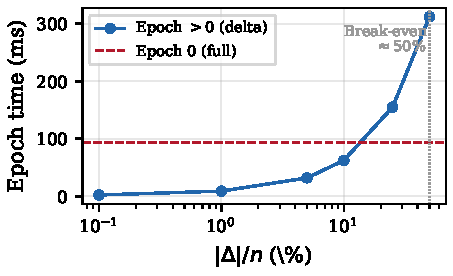
\includegraphics[width=0.8\columnwidth]{png/fig_delta_sweep.pdf}
\caption{Epoch time vs.\ delta ratio ($n = 2^{16}$, LAN). Break-even occurs at
$|\Delta|/n \approx 50\%$; below this threshold, FUPSU provides savings.}
\label{fig:delta}
\end{figure}

Fig.~\ref{fig:delta} shows epoch time as a function of the delta ratio
$|\Delta|/n$, at fixed $n = 2^{16}$ under LAN. The break-even point where
delta IBLT outperforms full re-encoding occurs at $|\Delta|/n \approx 50\%$;
below this threshold, FUPSU provides communication savings.

% ============================================================
\section{Full UC Security Proofs}
\label{sec:full-proofs}

\subsection{Full UC Security Proof}
\label{sec:full-proof}
% ============================================================

This appendix provides the complete UC security proof referenced in
Section~\ref{sec:security}. We give the full simulator construction, prove
all hybrid transitions, and establish the composition theorem.

\subsection{Complete Simulator Construction}

\begin{framed}
\noindent\textbf{Simulator $\cS$ for $\Pi_{\mathsf{fupsu}}$}

\smallskip\noindent\textbf{Input:} Access to $\cF_{\mathsf{updPSU}}$ and
$\cA$ (corrupting $P_0$ at epoch $\tau$).

\smallskip\noindent\textbf{Internal State:}
\begin{itemize}
\item $\tilde{Y}_t$: simulated $P_1$ set for each epoch $t$
\item $\tilde{K}^S_t \in \{0,1\}^\kappa$: simulated encryption key
\item $\widetilde{\mathsf{CT}}^{(t)}_S$: simulated ciphertext
\item $\tilde{\sigma}_{\mathsf{VOLE}}$, $\tilde{\sigma}_{\mathsf{OKVS}}$:
simulated VOLE and OKVS states
\end{itemize}

\smallskip\noindent\textbf{Procedure:}

\smallskip\noindent\textit{Initialization} ($t = 0$):
\begin{enumerate}
\item Sample $\tilde{K}^S_0, \tilde{K}^C_0 \sample \{0,1\}^\kappa$.
\item Initialize empty IBLTs for both parties.
\item Simulate VOLE setup: $\tilde{\sigma}_{\mathsf{VOLE}} \leftarrow
\textsf{SimVOLE}(1^\kappa)$. In the $\cF_{\mathsf{VOLE}}$-hybrid model,
$\cS$ simply records the ideal VOLE handles.
\end{enumerate}

\smallskip\noindent\textit{Per-Epoch Simulation} (epoch $t < \tau$):
\begin{enumerate}
\item Receive $X_{\cup,t}$ from $\cF_{\mathsf{updPSU}}$; receive $X_t$ (as
$P_0$'s input) from $\cZ$ through $\cA$.
\item Compute $\tilde{Y}_t \leftarrow X_{\cup,t} \setminus X_t$. By
construction, $X_t \cup \tilde{Y}_t = X_{\cup,t}$.
\item \textbf{Simulate UnionPeel.} Compute the virtual union IBLT:
$\mathsf{IBLT}_\cup \leftarrow \Encode(X_{\cup,t})$. Run the full
$\List(\mathsf{IBLT}_\cup)$ algorithm to obtain the peeling trace---the
ordered sequence of peeled elements and their originating cells
$(v_1, (i_1, j_1)), (v_2, (i_2, j_2)), \dots$

\item \textbf{Program ideal OT.} For each cell $(i,j)$ in the query set
$Q^{(r)}$ at iteration $r$, the ideal $\cF_{\mathsf{OT}}$ receives $P_0$'s
choice bit $c_{i,j}$ and $P_1$'s messages $(m_0, m_1)$. $\cS$ programs the
output to match the peeling trace:
\begin{itemize}
\item If the peeled element $v_{i,j}$ is unique to $P_0$
($\mathsf{cnt}_C = 1, \mathsf{cnt}_S = 0$): the 1-out-of-2 OT returns
$f_{i,j} \leftarrow m_{c_{i,j}}$ such that the subsequent computation
yields $v_{i,j} = \mathsf{sum}_C[i][j]$.
\item If $v_{i,j}$ is unique to $P_1$
($\mathsf{cnt}_C = 0, \mathsf{cnt}_S = 1$): the OT returns
$f_{i,j} \leftarrow \mathsf{sum}_S[i][j]$ from $P_1$'s message.
\item If $v_{i,j}$ is shared ($\mathsf{cnt}_C = \mathsf{cnt}_S = 1,
\mathsf{sum}_C = \mathsf{sum}_S$): the 1-out-of-3 OT result selection
returns $\mathsf{sum}_C[i][j]$.
\end{itemize}
$\cS$ records the programmed outputs in its local OT transcript store.

\item \textbf{Program ideal OPRF.} For each cell $(i,j)$, $\cS$ receives
$P_1$'s OPRF query $z_{i,j}$ and must produce tag $y_{i,j}$. If
$\mathsf{cnt}_C = 1$ and $\mathsf{sum}_C = z_{i,j}$ (equality case), $\cS$
programs $y_{i,j} \leftarrow F_k(\mathsf{sum}_C[i][j])$ using the known
OPRF key. Otherwise, $\cS$ outputs a uniformly random tag. This
programming is always possible because $\cS$ knows the full
$\mathsf{IBLT}_\cup$ and can precompute the equality conditions.

\item \textbf{Simulate ciphertext.} Sample $\tilde{K}^S_t \sample
\{0,1\}^\kappa$ (independent random). Encrypt a dummy IBLT of the
appropriate size: $\widetilde{\mathsf{CT}}^{(t)}_S \leftarrow
\SE.\Enc(\tilde{K}^S_t, N_S, 0^{|\mathsf{IBLT}_S|})$.

\item Simulate erasure: overwrite $\tilde{K}^S_{t-1}$ with zeros.
\end{enumerate}

\smallskip\noindent\textit{Corruption Handling} (epoch $t = \tau$):
\begin{enumerate}
\item $\cF_{\mathsf{updPSU}}$ sends $(X_\tau, K^C_\tau)$ to $\cS$.
\item $\cS$ delivers $(X_\tau, K^C_\tau)$ to $\cA$ as $P_0$'s internal
state.
\item $\cS$ continues simulating $P_1$ for epochs $t \geq \tau$ using the
same per-epoch procedure as above.
\end{enumerate}
\end{framed}

\subsection{Hybrid Argument: Full Proofs}

We prove Theorem~\ref{thm:main} via three hybrid simulators.

\begin{lemma}[Random Keys]\label{lem:hyb1-full}
$|\Pr[\cZ(\cS_1)=1] - \Pr[\cZ(\cS_0)=1]| \leq T \cdot
\mathsf{Adv}^{\mathsf{PRF}}_{F}(\kappa)$.
\end{lemma}

\begin{proof}
We construct a reduction $\cB$ to the PRF security of
$F = \mathsf{HMAC\text{-}SHA256}$. $\cB$ receives oracle access to either
$F(K, \cdot)$ (real PRF) or a truly random function $R(\cdot)$.

$\cB$ simulates the protocol execution for $\cZ$ using the hybrid
construction $\cS_1$, with the following modification for epoch $t$:
instead of sampling $\tilde{K}^S_t \sample \{0,1\}^\kappa$, it queries the
oracle on the fixed domain separator $c$: $\tilde{K}^S_t \leftarrow
\mathcal{O}(c)$.

If $\mathcal{O} = F(K, \cdot)$, then $\tilde{K}^S_t = F(K, c)$.
Combined with the real key chain starting from $K^S_0 = K$, this produces
exactly the key distribution of $\cS_0$ (real protocol).

If $\mathcal{O} = R(\cdot)$, then $\tilde{K}^S_t = R(c)$ is independent
of $K$ and of all other keys, producing exactly the distribution of
$\cS_1$ (random keys).

$\cB$ outputs whatever $\cZ$ outputs. The distinguishing advantage of
$\cB$ is exactly $|\Pr[\cZ(\cS_1)=1] - \Pr[\cZ(\cS_0)=1]|$, which is
bounded by $\mathsf{Adv}^{\mathsf{PRF}}_{F}(\kappa)$ for a single epoch.
Summing over $T$ epochs via a standard hybrid argument yields the $T
\cdot \mathsf{Adv}^{\mathsf{PRF}}_{F}(\kappa)$ bound.
\end{proof}

\begin{lemma}[Dummy Ciphertexts]\label{lem:hyb2-full}
$|\Pr[\cZ(\cS_{1.5})=1] - \Pr[\cZ(\cS_1)=1]| \leq T \cdot
\mathsf{Adv}^{\mathsf{IND\text{-}CPA}}_{\SE}(\kappa)$.
\end{lemma}

\begin{proof}
Analogous to Lemma~\ref{lem:hyb1-full}. For each ciphertext, replace the
$\SE$ keystream $\SE(\tilde{K}^S_t, N_S)$ with a truly random
string of the same length. Under the IND-CPA security of $\SE$, the
distributions are indistinguishable with advantage $\leq
\mathsf{Adv}^{\mathsf{PRG}}(\kappa)$ per ciphertext, and $\leq T \cdot
\mathsf{Adv}^{\mathsf{PRG}}(\kappa)$ over $T$ epochs. Note that
$\tilde{K}^S_t$ is already independent random (from Lemma~\ref{lem:hyb1-full}),
so the PRG reduction is straightforward.
\end{proof}

\begin{lemma}[Simulated Inputs]\label{lem:hyb3-full}
$\Pr[\cZ(\cS_2)=1] = \Pr[\cZ(\cS_{1.5})=1]$.
\end{lemma}

\begin{proof}
In both $\cS_{1.5}$ and $\cS_2$, $P_1$'s keys are independent random and
the IBLT ciphertexts are encryptions of the all-zero string. The only
difference is the content of $P_1$'s IBLT fed into
$\Pi_{\mathsf{UnionPeel}}$.

By Theorem~\ref{thm:upeel} (Union Peel Equivalence),
$\uPeel(\mathsf{IBLT}_C, \mathsf{IBLT}_S, i, j) =
\Peel(\mathsf{IBLT}_\cup, i, j)$ where $\mathsf{IBLT}_\cup =
\mathsf{IBLT}_C \oplus \mathsf{IBLT}_S$. The virtual union depends only
on $X_t \cup Y_t$, which equals $X_t \cup \tilde{Y}_t = X_{\cup,t}$ by
construction of $\tilde{Y}_t$. Therefore the peeling outputs---and hence
the entire protocol transcript in the
$(\cF_{\mathsf{OPRF}}, \cF_{\mathsf{OT}})$-hybrid model---are identical
in distribution for $Y_t$ and $\tilde{Y}_t$.

After corruption at epoch $\tau$, $\cF_{\mathsf{updPSU}}$ reveals
$(X_\tau, K^C_\tau)$. The simulated view for $t < \tau$ used only
$X_{\cup,t}$, which $\cS$ received from $\cF_{\mathsf{updPSU}}$. No
inconsistency arises because $\cS$ never committed to a specific $Y_t$
beyond what $X_{\cup,t}$ implies. The view is perfectly identical.
\end{proof}

Combining Lemmas~\ref{lem:hyb1-full}-\ref{lem:hyb3-full}, the total
distinguishing advantage between the real world ($\cS_0$) and the ideal
world ($\cS_2$) is bounded by $T \cdot (\mathsf{Adv}^{\mathsf{PRF}}(\kappa
+ \mathsf{Adv}^{\mathsf{PRG}}(\kappa)) \leq \negl(\kappa)$, completing the
proof of Theorem~\ref{thm:main}. \hfill$\square$

\subsection{UC Composition: Formal Statement}

\begin{theorem}[UC Composition]\label{thm:composition}
Let $\Pi_{\mathsf{epoch}}$ be a protocol that UC-realizes $\cF_{\mathsf{psu}}$
in the $(\cF_{\mathsf{OPRF}}, \cF_{\mathsf{OT}})$-hybrid model, and let
$\Pi_{\mathsf{key}}$ be a protocol that UC-realizes $\cF_{\mathsf{fwKey}}$.
Then the parallel composition $\Pi_{\mathsf{epoch}} \parallel
\Pi_{\mathsf{key}}$ UC-realizes $\cF_{\mathsf{updPSU}}$ in the same hybrid
model.
\end{theorem}

\begin{proof}[Proof sketch]
By the universal composition theorem~\cite{Can01}, it suffices to exhibit a
simulator for $\cF_{\mathsf{updPSU}}$ given simulators for $\cF_{\mathsf{psu}}$
and $\cF_{\mathsf{fwKey}}$. The construction is modular: the per-epoch
simulator $\cS_{\mathsf{epoch}}$ (from Piske and Trieu~\cite{PT26}) handles
all OT/OPRF interactions within each epoch, receiving $X_{\cup,t}$ from
$\cF_{\mathsf{updPSU}}$. The key management simulator $\cS_{\mathsf{key}}$
samples independent random keys for $t < \tau$ (indistinguishable from PRF
outputs by PRF security) and delivers the current key upon corruption. The
composition is a standard application of the UC theorem, requiring no new
cryptographic assumptions.
\end{proof}

% ============================================================
\section{Self-Healing Key Chains}
\label{sec:selfheal}
% ============================================================

FUPSU achieves forward security but not post-compromise security. We present
a protocol extension achieving \emph{self-healing} with \textbf{zero additional
communication}, protecting against single-party compromise.

\textbf{Key insight: the union output as a nonce source.}
At each epoch, both parties learn $X_{\cup,t}$. Critically, \emph{neither
party knows which elements were contributed by the other}. From $P_0$'s
perspective, $X_{\cup,t} \setminus X_t$ is unpredictable (it consists of
$P_1$'s exclusive elements). This entropy can serve as a fresh random nonce.

\textbf{Protocol modification.}
Replace the key update with:
\[
K^b_t \leftarrow \PRF(K^b_{t-1},\; c \concat H(X_{\cup,t})),
\]
where $H$ is a collision-resistant hash. Both parties compute $H(X_{\cup,t})$
locally---no additional round, no additional communication.

\textbf{Security argument.}
Consider compromise at epoch $\tau$. The adversary learns $K^b_\tau$ and
$X_{\cup,\tau}$. To compute $K^b_{\tau+1}$, the adversary needs
$H(X_{\cup,\tau+1})$ at the next epoch. But $X_{\cup,\tau+1} \setminus
X_{\cup,\tau}$ contains deltas applied by the \emph{honest party}, which the
adversary cannot predict. Therefore:
\begin{itemize}
\item Before compromise: adversary without $X_{\cup,t}$ (forward privacy
prevents decryption) cannot compute $K^b_{t+1}$.
\item After compromise detected: the honest party's delta introduces fresh
entropy, healing the chain.
\item Healing time: one epoch after non-trivial honest update.
\end{itemize}

\textbf{Security bound.}
For exclusive set size $|X_{\cup,t} \setminus X_b| \geq q$, min-entropy:
$\log\binom{|U|-|X_b|}{q} \geq q(\sigma - \log|U|)$ bits. With $q = 1$ and
$\sigma \geq 128$, this exceeds $\kappa = 128$, giving single-epoch healing.

\textbf{Practical considerations.}
Healing requires the honest party to make a non-trivial update. \emph{Entropy
decay}: if the adversary observed $T$ prior unions, the honest party's
exclusive set may be reduced, increasing expected healing time to
$O(|U|/|\text{exclusive}|)$ epochs. This construction shows that PSU's
inherent output entropy can be leveraged for cryptographic self-healing
without additional communication, a property unique to updatable PSU among
secure computation primitives.

\subsection{Comparison with DH-Based Ratchets}

Unlike DH-based ratchets~\cite{Signal} which require an extra round per
epoch for ephemeral key exchange, the self-healing construction uses only
the union output entropy (zero additional communication). Healing occurs
in a single epoch whenever the honest party makes a non-trivial
update---a condition naturally satisfied in deployments with regular
activity (e.g., daily IoC feeds). The approach is complementary to DH:
both can be combined for defense in depth.

% ============================================================
\section{Additional Material}
\label{sec:additional}
% ============================================================

\subsection{Experimental Validation of the Cascade Bound}

We experimentally validated the cascade bound across the full parameter
range. Table~1 in Section~\ref{sec:eval} shows that the
observed cascade ratio is $\approx 1.95 \times k|\Delta|$ (averaged over
20 trials), well within the $2 \times k|\Delta|$ theoretical bound. The
ratio is stable across all values of $n$ and $|\Delta|$, confirming that
the $2$-core emptiness assumption holds in practice for the chosen IBLT
parameters.

The cascade ratio approaches $1.0 \times k|\Delta|$ as $|\Delta|/n \to
0$, since the probability of hash collisions among delta elements
vanishes with decreasing delta density. At $|\Delta|/n = 0.1\%$, we
observe cascade ratios of $1.01$--$1.05 \times k|\Delta|$, indicating
that the delta elements are essentially isolated in the IBLT hypergraph.

% ============================================================
\subsection{Deployment Considerations}
\label{sec:deployment}

FUPSU is most beneficial when: (i)~sets evolve incrementally with
$|\Delta| \ll n$ (the update ratio is small); (ii)~frequent
recomputation of the union is required (low-latency requirements);
(iii)~sensitive historical data must be protected against key compromise
(regulatory compliance); (iv)~network bandwidth is constrained (WAN or
low-bandwidth links). In these scenarios, FUPSU provides substantial
communication savings ($1{,}856\times$ at $|\Delta|=2^{10}$ at $0.1\%$ update ratio on $n=2^{20}$) and forward
privacy with negligible overhead.

FUPSU provides limited benefit when: (i)~the update ratio is high
($|\Delta|/n > 50\%$, see Fig.~\ref{fig:delta}); (ii)~the
deployment is on a high-bandwidth LAN where IBLT peeling computation
dominates; (iii)~forward privacy is not required and a static protocol
suffices.

\smallskip\noindent\textbf{Scalability.}
For $n > 2^{20}$, rateless IBLTs~\cite{YGA24}, sharding, and
multi-threading compose naturally with FUPSU's linear delta mechanism.

\end{document}

\end{document}
